\documentclass[hidelinks, 12pt]{style} 

\usepackage[utf8]{inputenc}
\usepackage{fancyhdr} 
\pagestyle{fancy}
\usepackage{amssymb}
\usepackage{caption}
\usepackage{subcaption}
\usepackage{float}
\graphicspath{{Images/}} 
\usepackage[backend=biber,style=phys]{biblatex}
\newtheorem{definition}{Definition}
\usepackage{tocbibind}
\usepackage{tabularx}
\usepackage{amsmath}
\usepackage[toc,title,page]{appendix}
\usepackage{hyperref}
\usepackage{minted}
\usepackage{blindtext}
\usepackage{url}
\usepackage{epigraph}
\usepackage{tikz}
\usepackage[intoc]{nomencl}
\usepackage[makeroom]{cancel}
\usepackage{algpseudocode}
\usepackage{algorithm}
\usepackage{chemfig}
\usetikzlibrary{quotes,arrows.meta}
\makenomenclature
\addbibresource{references.bib}

\usepackage{etoolbox}
\renewcommand\nomgroup[1]{%
  \item[\bfseries
  \ifstrequal{#1}{A}{Greek Letters}{}
  \ifstrequal{#1}{B}{Roman Letters}{}
]}

% This will add the units
%----------------------------------------------
\newcommand{\nomunit}[1]{%
\renewcommand{\nomentryend}{\hspace*{\fill}#1}}
%----------------------------------------------

\title{AMSIMP: An Open Source Implementation to Simulating Tropospheric and Stratospheric Dynamics on a Synoptic Scale} 

\author{Conor Casey} 
\college{Teacher: Ms. Abbott} 

\degree{Chemical, Physical, and Mathematical Sciences} 
\degreedate{Stand 2300 - BTYSTE 2020} 

\begin{document}

\maketitle

\clearpage\mbox{}\clearpage

\pagenumbering{roman}

\chapter*{
\centering
    ``All stable processes we shall predict. All unstable processes we shall control.”
\\[5pt]
\rightline{{\rm --- Jean-Baptiste Lamarack}}
}

\chapter*{Abstract}
\addcontentsline{toc}{chapter}{Abstract}
This report hypothesises that it is possible to create an open-source implementation to simulating tropospheric and stratospheric dynamics on a synoptic scale, that such software is consistent and reliable, and that the software consists of high-quality source code. Firstly, this report explains, and derives a series of relevant equations for simulating atmospheric dynamics on a synoptic scale.

Following this process, the software was developed and released onto the open-source platform, GitHub. To prove the hypothesis, it was determined that a series of appropriate benchmarks would be carried out in the areas of performance, accuracy, and code quality. The performance benchmark would demonstrate whether or not the software has consistent and reliable performance, the accuracy benchmark would highlight whether or not the forecasts produced by the software has a reasonable level of accuracy, and the code quality benchmark would indicate whether or not the source code of the software was of high quality.

In regards to the performance benchmark, the time it took to generate a four-day forecast was measured. This benchmark was carried out on three completely different machines, with a sample size of ten measurements on each machine. The statistical analysis of the results found that the mean coefficient of variation ($\frac{\sigma}{\bar{x}}$) was approximately, 0.04. This signified that there was a low variation in execution time, proving that the performance of the software was consistent and reliable.

In regards to the accuracy benchmark, it showed that a four-day forecast produced software had a mean absolute percentage error of approximately 1.56 \%, and a median absolute percentage error was approximately 0.81 \%. This shows that the forecast produced by the software is accurate, which further proves that its consistency and reliability. 

In regards to the code accuracy benchmark, two distinct benchmarks were carried out. The first benchmark indicated that the software consists of high quality source code, as it received a numerical rating of 7.32 from Pylint which corresponds to an interpretation of `Great Code!'. The second benchmark indicated that the software had a code coverage of approximately 98 \%. This signifies that the software has a lower chance of containing undetected bugs, ultimately demonstrating that the quality of the source code is high. Both of these benchmarks clearly highlight that the software consists of high quality source code. 

All aspects of the hypothesis's statement have been verified, hence, the hypothesis as originally stated can be accepted.

\chapter*{Acknowledgements}
\addcontentsline{toc}{chapter}{Acknowledgements}
\paragraph{Ms. Abbott} First and foremost, I would like to express my immense gratitude to my science teacher, Ms Abbott. Over the past two years, she has provided me with an unwavering amount of support and faith in any scientific endeavour I have pursued, even when I didn't have much of the latter myself. She’s always been there for me, both academically and personally. She has been a source of comfort and refuge, even in the most difficult of times. That is also not to mention the fact that she is probably the most fantastic teacher that walks the face of the planet. She would probably say I am being entirely hyperbolic, even though I wholeheartedly insist I am not. This is not a belief, it's a law of nature! Although, she does have a pathological habit of refusing to take any thanks I give her whatsoever. She is an amazing human being, even if I cannot express how grateful I am in words all the time. So, just to emphasise one last time:  THANK YOU SO, SO, SO MUCH!

\paragraph{Hannah Coombs} I would like to take the opportunity to thank my dear friend, Hannah Coombs. Over these past few years, she has always been/continues to be extremely kind, and supportive to me. She has helped me gain the confidence that I was once lacking, and has made me a better person. Although she didn't provide any assistance for this particular project, I am forever indebted to her.

\paragraph{Dr. Doireann O'Kiely} I would like to thank Dr. Doireann O'Kiely for the guidance she offered for the initial phase of the project, and also providing support throughout the entirety of the project.

\paragraph{Mr. Healy, and Ms. Foley-Hayes}
I would like to thank Mr. Healy, and Ms. Foley-Hayes, our Principal and Vice Principal, for their support in relation to funding, incorporating various different ideas into my project, and generally providing all the assistance I needed.

\paragraph{Institute of Physics}
I would like to thank the the Institute of Physics for providing the physical copy of the book, `Physics of the Atmosphere' by Rodrigo Caballero.

\paragraph{Parents} Due to an error made during the printing process, the acknowledgement to my parents, Timmy and Frances to whom I owe everything, was unfortunately not included. I would like to take the opportunity to express how grateful I am for all the support, help, guidance, feedback and love that they have provided me over these many years. I will be eternally grateful for this.

\tableofcontents

\listoffigures

% Nomenclatures
\mbox{}

\nomenclature[A, 01]{$\eta$}{Absolute Vorticity  
  \nomunit{$rad \cdot s^{-1}$}}
\nomenclature[A, 02]{$\theta$}{Potential Temperature
  \nomunit{$K$}}
\nomenclature[A, 03]{$\lambda$}{Longitude 
  \nomunit{$^{\circ}$}}
\nomenclature[A, 04]{$\Pi$}{Exner Function
  \nomunit{$\frac{K}{K}$}}
\nomenclature[A, 05]{$\sigma$}{Sigma Vertical Coordinate
  \nomunit{$\frac{hPa}{hPa}$}}
\nomenclature[A, 6]{$\Phi$}{Geopotential Height 
  \nomunit{$m$}}
\nomenclature[A, 07]{$\phi$}{Latitude 
  \nomunit{$^{\circ}$}}
\nomenclature[A, 08]{$\rho$}{Density 
  \nomunit{$kg \cdot m^{-3}$}}
\nomenclature[A, 09]{$\omega$}{Vertical Velocity 
  \nomunit{$Pa \cdot s^{-1}$}}
\nomenclature[A, 10]{$\Omega$}{Angular Rotation Rate of Earth
  \nomunit{$7.29246206 \cdot 10^{-5}\, rad \cdot s^{-1}$}}

\nomenclature[B, 01]{$a$}{Earth mean radius
  \nomunit{$6378100 m$}}
\nomenclature[B, 02]{$c_p$}{Specific Heat Capacity on a Constant Pressure Surface
  \nomunit{$1004, J \cdot kg^{-1} \cdot K^{-1}$}}
\nomenclature[B, 03]{$e$}{Saturated Vapour Pressure
  \nomunit{$hPa$}}
\nomenclature[B, 04]{$F$}{Coriolis Force
  \nomunit{$rad \cdot s^{-1}$}}
\nomenclature[B, 04]{$f$}{Coriolis Parameter
  \nomunit{$rad \cdot s^{-1}$}}
\nomenclature[B, 05]{$g$}{Gravitation Acceleration
  \nomunit{$m \cdot s^{-2}$}}
\nomenclature[B, 06]{$m$}{Mixing Ratio
  \nomunit{$\frac{kg}{kg}$}}
\nomenclature[B, 07]{$h$}{Pressure Thickness
  \nomunit{$m$}}
\nomenclature[B, 08]{$p$}{Pressure
  \nomunit{$hPa$}}
\nomenclature[B, 09]{$R$}{Specific Gas Constant for Dry Air
  \nomunit{$287, J \cdot kg^{-1} \cdot K^{-1}$}}
\nomenclature[B, 10]{$T$}{Temperature
  \nomunit{$K$}}
\nomenclature[B, 11]{$t$}{Time
  \nomunit{$s$}}
\nomenclature[B, 12]{$u$}{Zonal Wind
  \nomunit{$m \cdot s^{-1}$}}
\nomenclature[B, 13]{$v$}{Meridional Wind
  \nomunit{$m \cdot s^{-1}$}}
\nomenclature[B, 14]{$W$}{Precipitable Water
  \nomunit{$mm$}}
\nomenclature[B, 15]{$x, y$}{Horizontal Distances
  \nomunit{$m$}}
\nomenclature[B, 16]{$z$}{Vertical Distance
  \nomunit{$m$}}
 
\printnomenclature

\chapter{Introduction} 
\pagenumbering{arabic} 
\epigraph{``Yes, it is easy to see that nearly six years of magical education has not been wasted on you ... Ghosts are transparent"}{Severus Snape}

Numerical Weather Prediction focuses on taking current observations of weather and processing this data with computer models to forecast the future state of weather. Knowing the current state of weather is just as important as the numerical computer models processing the data. Current weather observations serve as input to the numerical computer models through a process known as data assimilation to produce outputs of temperature, precipitation, and hundreds of other meteorological elements from the oceans to the top of the atmosphere\cite{nwp_introduction}. 

However, weather prediction is not all that it could be. For example, you should remember Hurricane Sandy, which hit New York in 2012. The American Global Forecast System predicted it would not even reach the mainland! This, of course, was wrong, and as a result, 285 people died and 68.7 billion dollars worth of damage was done. But, why is weather forecasting so hard? Forecasting today is done by physical modelling. This means we know the equations that govern weather systems, but we can’t solve them exactly. Instead, we approximate them.  Weather agencies take reams of raw data, feed it into supercomputers, and just number crunch and number crunch. As you can imagine, this requires a significant amount of computational resources. This is not only a cost issue, it also inhibits our ability to produce forecasts of a high temporal resolution; which can be significantly important in predicting extreme weather events, such as tornadoes.

\section{Development of the Idea}
I think it is extremely difficult to pinpoint exactly where the idea originated from; on reflection, however, the spark which really ignited the flame for this project came from a deep interest in the study of the atmosphere and by extension atmospheric science. I initially became interested in this topic based on two distinct factors. 

I became interested in the area of atmospheric science from watching a YouTuber named, Dr. Simon Clark. Dr. Simon Clark recently completed a PhD in theoretical atmospheric physics, researching dynamical stratosphere-troposphere coupling, and made a vlog series documenting his experiences. I was extremely intrigued by this series, with keen interest in his videos explaining his research. These videos captivated me and ultimately led me to reading his thesis (titled Quasi-geostrophic influence of the polar stratosphere on the troposphere)\cite{simonclark}.

Secondly, my interest also came from my concern over human caused climate change. I was extremely fascinated by how a gas, such as carbon dioxide, could capture so much more heat than oxygen, even though there is a higher concentration of oxygen in the atmosphere. This ultimately led to the original idea for this project: creating a computational simulation of both Earth and Venus, and using it to determine if Earth could become just as hellish and uninhabitable as Venus if the rate at which we were pumping carbon dioxide into the atmosphere remained constant. There was a few problems with this idea, primarily being that it would require a ridiculous amount of computational resources, and there was no way of ensuring it was accurate. This led me to narrow the scope of the project, and ultimately, I eventually settled on the idea of improving numerical weather prediction in some fashion. From my initial research, as I previously mentioned, atmospheric simulations required a significant amount of computational power. There have been fantastic developments in machine learning over the past decade, and I wanted to apply these advancements to the problem of weather forecasting. Through various discussions with experts in a wide variety of fields, I came to the conclusion that such an endeavour may be fruitful.

\section{Aims}
The principal aim of this project is to create a neural network architecture, which will reduce the amount of computational resources required to generate weather forecasts compared to traditional physics-based models; and one which will provide a similar level of performance when compared to physical models. Access to the source code of any given physics-based forecast system is also notoriously difficult, with enormous price tags being the norm to gain access to time critical weather information. My vision is to make better weather tools available to everyone. Once the software is created, it will be published on the open source platform, known as, GitHub. This will allow programmers, and atmospheric physicists alike to inspect the source code, and to contribute to the development of the software. The software will also be published on Anaconda Cloud. I did this in order to allow, with just a simple command, the installation of the software. I will also develop a series of documentation that will accompany the software, which will accumulate in the development of a website.

\begin{figure}[H]
    \centering
    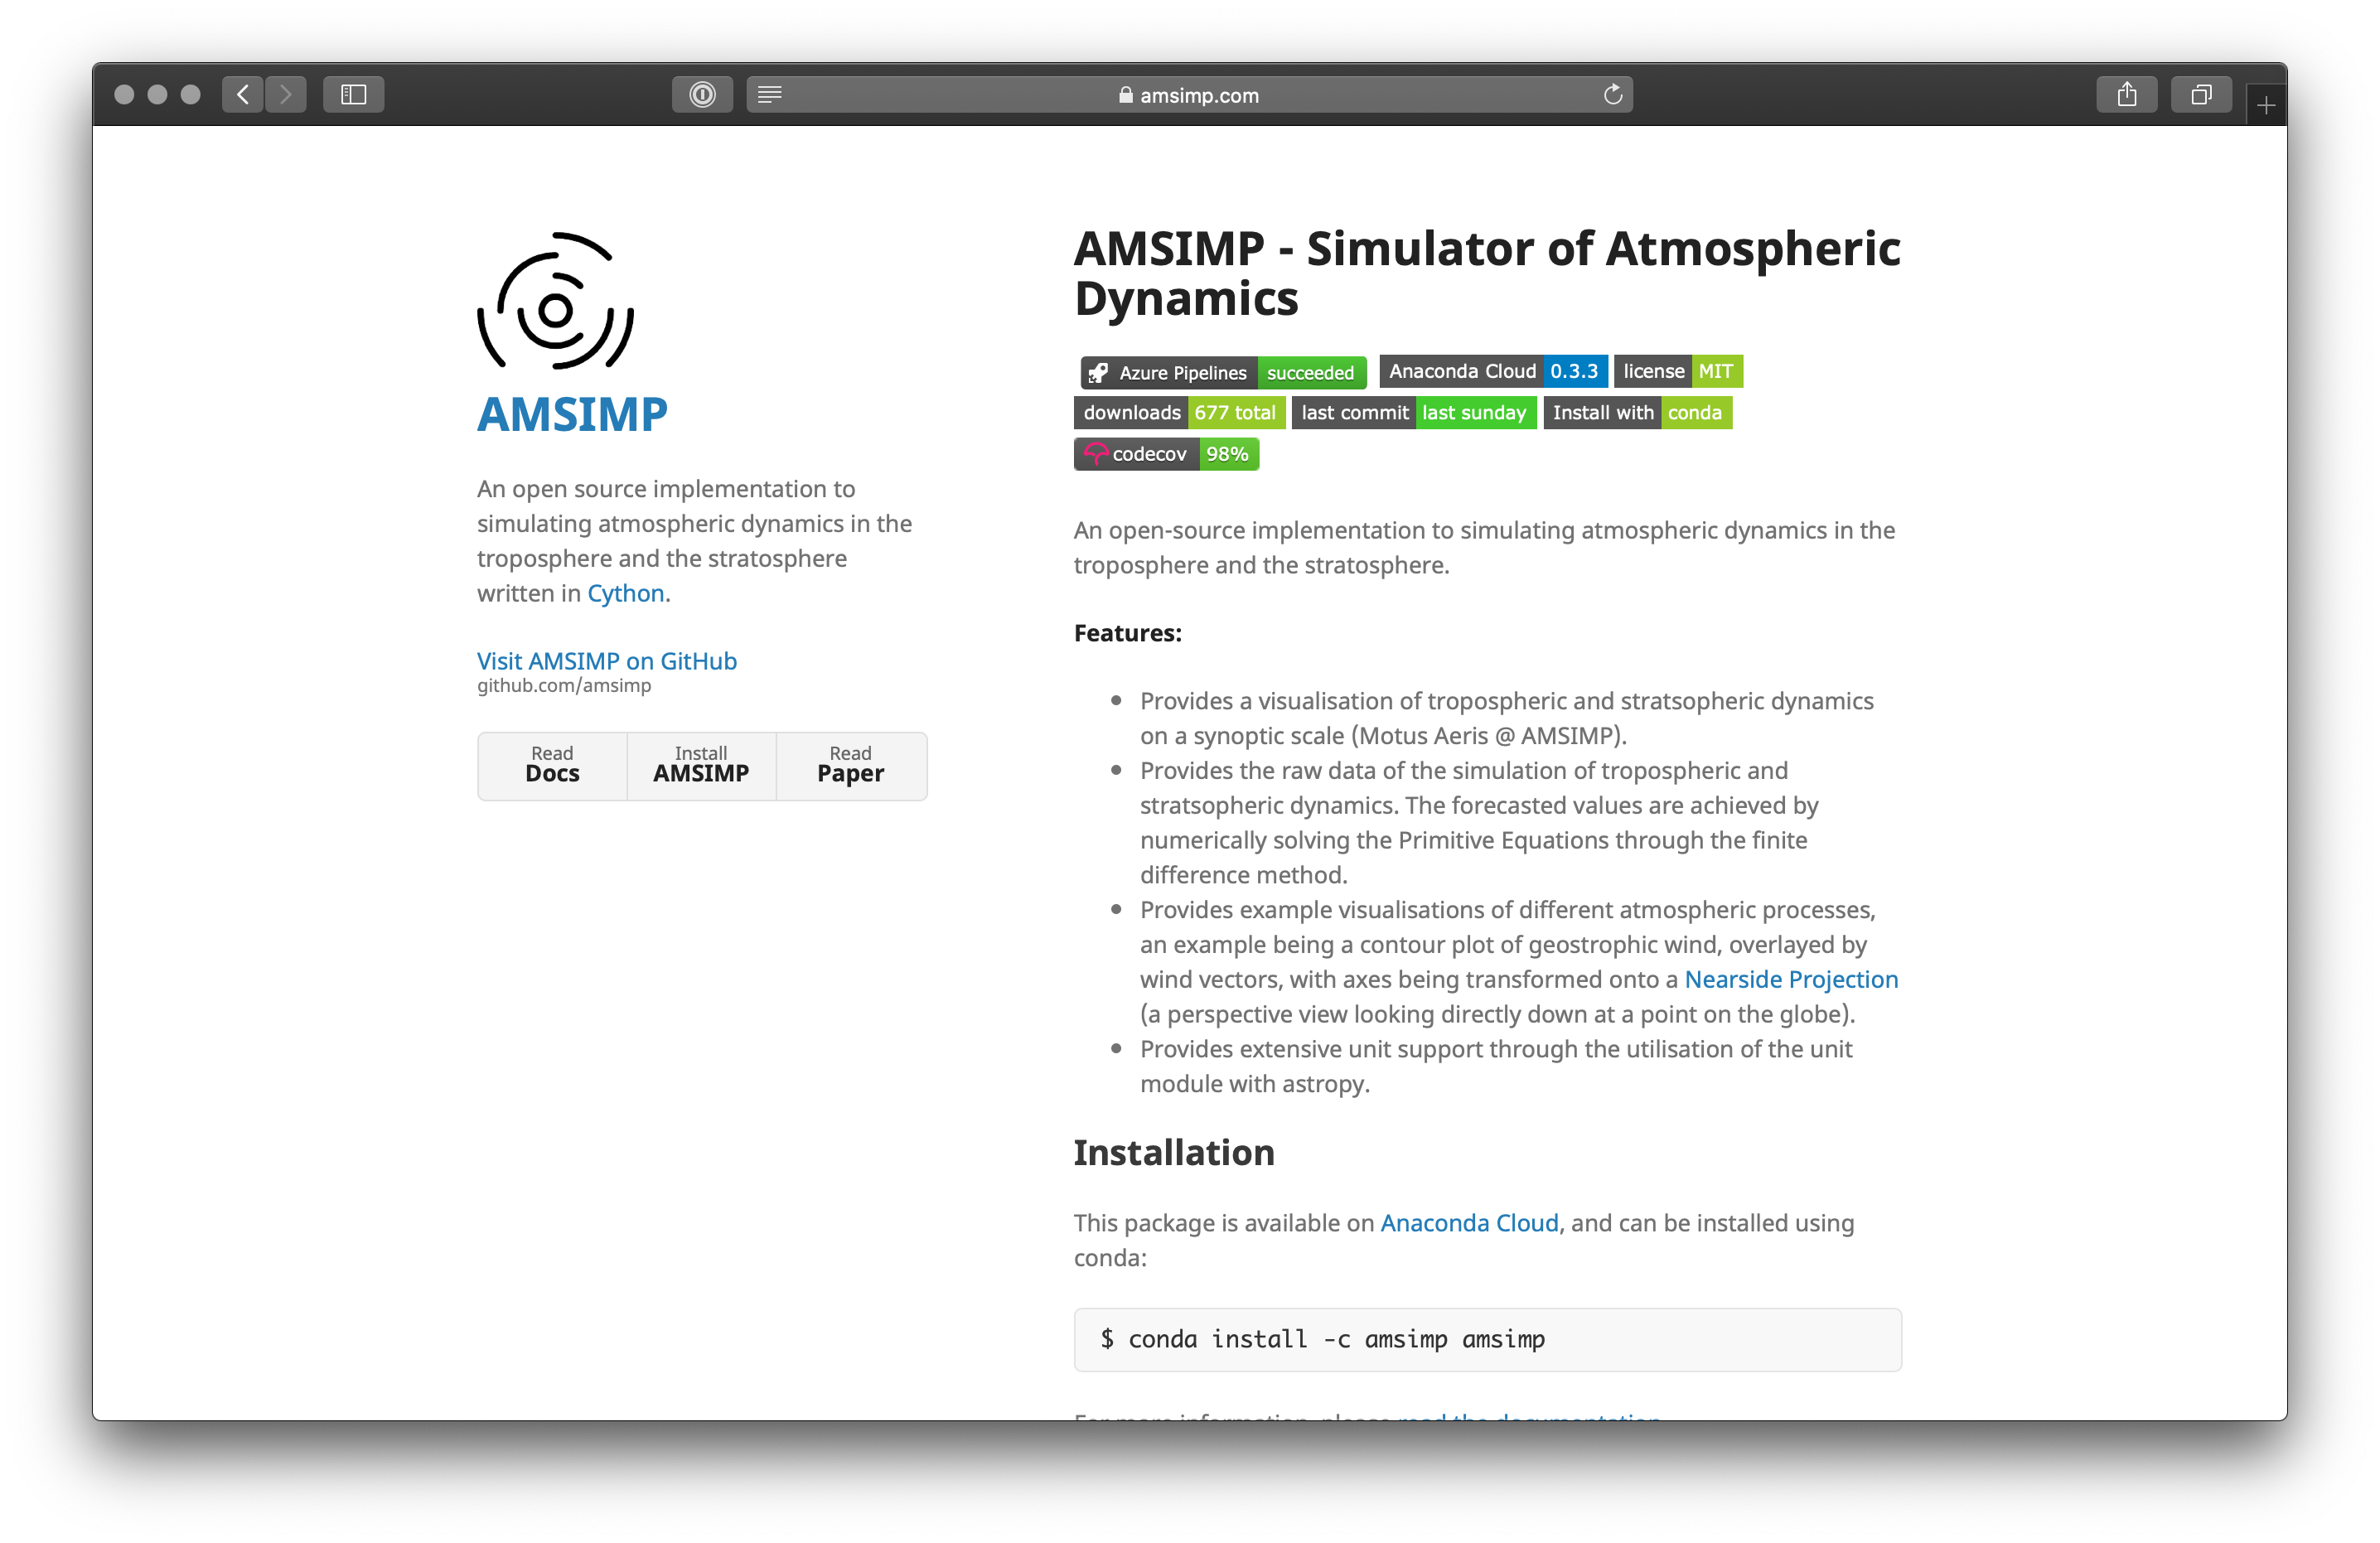
\includegraphics[width=.75\linewidth]{Images/website}
    \caption{A screenshot of the website for the software.}
    \label{website}
\end{figure}

\section{Organisation of this Work}
The work contained in this project book is broken down into a number of different chapters:

\begin{itemize}
    \item Chapter \ref{architecture_chapter} discusses the various neural network architecture under consideration and the current implementation within the software.
    \item Chapter \ref{implementation_chapter} discusses some of the decisions made on the software development side of the project, such as, choosing an appropriate programming language for the task. 
    \item Chapter \ref{benchmarking_chapter} outlines the software benchmarking experiments to be carried out on the software.
    \item Chapter \ref{results_chapter} contains the results of the benchmarking described in the previous chapter.
    \item Chapter \ref{conclusion_chapter} reviews the results and outcomes of the project, discusses the limitations of the software, and lays out a road-map for the continued development and enhancement of the software. 
\end{itemize}


\chapter{Atmospheric Science}\label{2}
\epigraph{``Time will not slow down when something unpleasant lies ahead."}{Harry Potter}

\begin{definition}
The atmosphere is a continuous stratified fluid stretching from the surface of the Earth to space, with a atmospheric density that decreases exponentially with altitude (see figure \ref{density}). It is held near to the surface of the planet by Earth's gravitational field. 
\end{definition}

The atmosphere consists of a mixture of gases, being mostly nitrogen, and oxygen. These two individual gases account for roughly 99\% of the atmospheric constituents. These gases are generally classified as well mixed. This ultimately means that these gases have long residual times, and as a result, the amount in which they are present in the atmosphere is essentially constant in space and time. These gases along with a spattering of other well mixed fixed gases are generally treated as a singular entity. This theoretical entity is called dry air (see table 1.1). On the side of variable constituents, water vapour is by far the most critical. At any given moment, water vapour can account for anything between 5\% of the atmosphere, and almost zero in the stratosphere. In fact, to an excellent approximation, the atmosphere can be thought of as two distinct entities, the aforementioned dry air, and water vapour\cite{iop}.

\begin{center}
\begin{tabular}{c c} 
 \hline
 Constituent & Number Fraction (\%) \\
 \hline
 Nitrogen ($N_2$) & 78.08 \\
 Oxygen ($O_2$) & 20.95 \\
 Argon ($Ar$) & 0.93 \\
 Carbon Dioxide ($CO_2$) & 0.038 \\
 Neon ($Ne$) & 0.001818 \\
 Helium ($He$) & 0.000524 \\
 Methane ($CH_4$) & 0.0001745 \\
 Krypton ($Kr$) & 0.000114 \\
 Hydrogen ($H_2$ & 0.000055 \\
\end{tabular}\par
\end{center}

\hfill

\begin{center}
\begin{tabular}{c c} 
 Water Vapour ($H_{2}O$) & 0 - 5 \\
 Ozone ($O_3$) & 0 - 0.00001 \\
 \hline
\end{tabular}\par
\bigskip
Table 1.1.: Composition of the Atmosphere.
\end{center}

In regards to a boundary between the atmosphere and outer space, there is no exact boundary, it just keeps getting less and less dense, until it ``blends" into space. One common convention, however, for such a boundary is 100,000 metres above mean sea level, the Kármán line\cite{simonclark}.


The atmosphere is divided into four distinct layers: the troposphere, the stratosphere, the mesosphere, and the thermosphere. These layers are defined and  characterised by their vertical temperature profile, essentially how temperature changes within them with increased altitude (see figure \ref{temp_profile}). Considering this project is specifically focused on atmospheric dynamics in the troposphere and the stratosphere, it will only be necessary to discuss these two layers. 

\begin{figure}[H]
    \centering
    \begin{subfigure}{.44\textwidth}
        \centering
        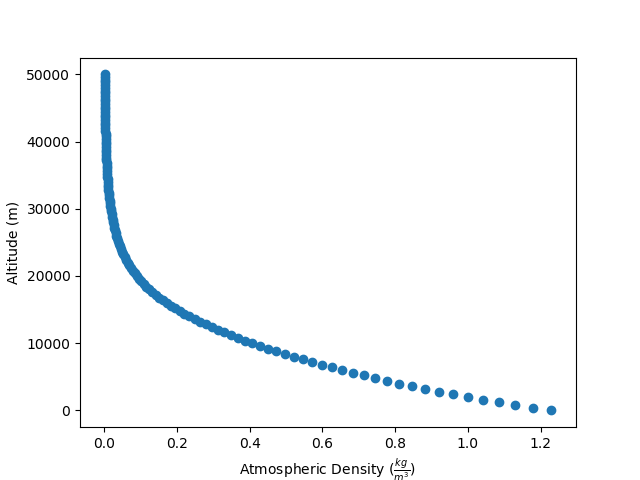
\includegraphics[width=\textwidth]{Images/vertical_density_profile}
        \caption{Vertical Profile of Atmospheric Density}
        \label{density}
    \end{subfigure}
    \hfill
    \begin{subfigure}{.44\textwidth}
        \centering
        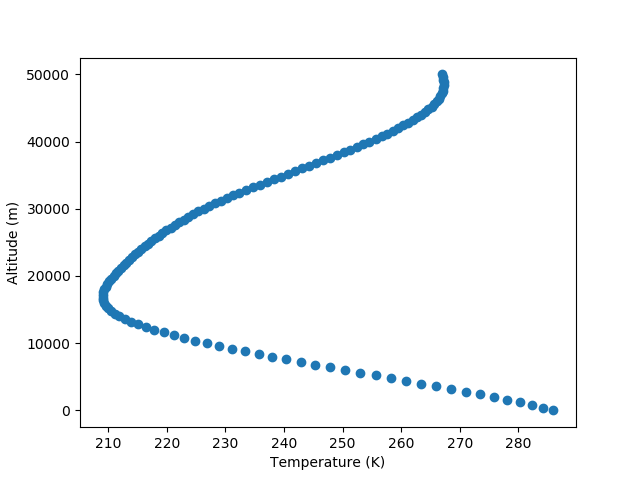
\includegraphics[width=\textwidth]{Images/vertical_temperature_profile.png}
        \caption{Vertical Profile of Temperature}
        \label{temp_profile}
    \end{subfigure}
    \caption{Vertical Profiles of the Troposphere and the Stratosphere}
\end{figure}

\section{Troposphere}
\subsection{Lower and Upper Troposphere}
The troposphere is the layer closest to the surface of the Earth, and rises to a global mean altitude of 11,000 metres. The depth of this layer is relatively thin, however, it contains approximately 80\% of the total overall mass of the atmosphere. 

Because the atmosphere is compressible, air molecules are more compact closer to the surface, thereby increasing the overall atmospheric density and pressure of the air at lower altitudes. Atmospheric pressure just like density decreases exponentially with an increase in altitude (see figure \ref{atmospheric_pressure_intro}). In the lower troposphere, the rate of pressure decrease is about 1000 Pascals for every 100 metres.

\begin{figure}[H]
    \centering
    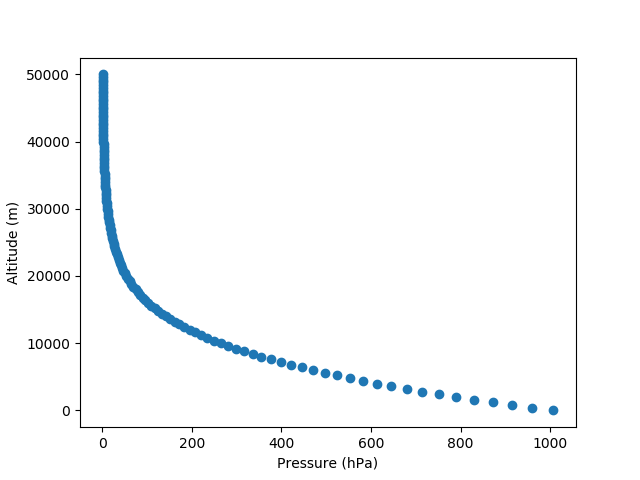
\includegraphics[width=.8\linewidth]{Images/vertical_pressure_profile}
    \caption{Vertical Profile of Atmospheric Pressure in the the Troposphere and the Stratosphere}
    \label{atmospheric_pressure_intro}
\end{figure}

Temperature in the troposphere decreases with altitude (with the exception of the tropopause), contrasting considerably between the lower and upper portions (again, see figure \ref{temp_profile}). Temperature in this particular layer is controlled by a variety of factors, including latitude, season, a location's distance from the ocean, and on, and on. Atmospheric scientists, however, use a concept called a standard atmosphere to present an average atmosphere\cite{temp_in_trop}. The global mean surface temperature is approximately 288.15 K, with the upper portion of the troposphere averaging around 216.65 K. The rate at which this temperature decreases is on average 0.0065 K per metre. Side note, the rate at which temperature increases, decreases, or remains constant on average is commonly called the normal lapse rate by atmospheric scientists.

The mean height of the troposphere varies considerably with latitude. In the tropics, the altitude of the troposphere is around 16,000 metres, but near the poles, this shrinks to about 8,000 metres.

Evidence suggests that the troposphere has undergone a significant rate of warming during the past century. The tropospheric temperature trend in the latter half of the 20th century is estimated at a 0.10 K increase per decade. This is primarily a result of the human-induced perturbation known as, climate change\cite{troposphere}.

\subsection{Tropopause}
At a mean altitude of approximately 11,000 metres, the tropopause commences. This is typically determined by the vertical temperature profile (see figure \ref{temp_profile}). During this particular phase of the atmosphere, temperature remains approximately constant at around 216.65 K until about 32,000 metres above sea level at which point the stratosphere commences. The tropopause is turbulent and well mixed.

\section{Stratosphere}
The stratosphere, as mentioned previously is the second layer of atmosphere. Unlike the troposphere, temperature within the stratosphere increases with altitude. The increasing temperature in the stratosphere is caused by the presence of a layer of ozone near an altitude of approximately 25,000 metres. The ozone molecules absorb high-energy ultraviolet electromagnetic radiation from the sun, which by extension, warms the atmosphere in this layer. The stratosphere is defined as the region between the tropopause and the level at which the maximum warming due to the presence of ozone takes place, which is at an altitude of about 50,000 metres. About 90\% of the ozone in the atmosphere is within this region. Its concentrations in the ozone layer are typically only 1 to 10 parts of ozone per 1 million parts of air\cite{mit}.

\begin{figure}[H]
    \centering
    \chemfig{O=[:50]O \textsuperscript{+}-[:-50]O \textsuperscript{-}}
    \caption{The chemical structure of the ozone atom, $O_3$}
    \label{ozone}
\end{figure}

As mentioned at the beginning of the chapter, the stratosphere consists of extremely dry air, and is by extension, lacking in water vapour. As a consequence, this layer has a low amount of clouds, with almost all clouds being located in the lower, more humid troposphere. This is due to a lack of vertical dynamics within the stratosphere. This also results in materials staying within this layer for long stretches of time. Major meteorite impacts can launch particles straight into the stratosphere attaining extremely high velocities. These particles then linger within this layer, for for months or years, sometimes altering the Earth's global climate significantly\cite{stratosphere}. An example of such an event was the meteorite impact than ultimately killed the dinosaurs. This event launched a significant amount of debris into the stratosphere, which ultimately accumulated, and resulted in a significant drop in global average temperature for the next few years succeeding the event. 

\section{Atmospheric Circulation}
In order for one to truly understand the equations that will be utilised to simulate atmospheric dynamics, it is necessary to examine how atmospheric circulation functions. 

\subsection{Global Heat Energy Budget}
The Global Heat Energy is the equilibrium between incoming and outgoing solar electromagnetic radiation. This incoming and outgoing electromagnetic radiation is known as insolation. 

\begin{definition}
Insolation is defined as the incoming solar electromagnetic radiation that is absorbed, or reflected by the atmosphere
\end{definition}

Approximately 50 \% of the insolation passes through the atmosphere and reaches the surface. Of that, about 46 \% is absorbed with the remainder being reflected. This particular form of reflection is known as the albedo of the Earth. The albedo of an object is just the extent to which that particular object reflects light. Some of the outgoing ultraviolet solar radiation is absorbed by greenhouses gases, such as carbon dioxide and water vapour. This is known as the greenhouse effect. Since the industrial revolution, the amount of greenhouses gases within the atmosphere has dramatically increased. This is resulting in a large amount of this outgoing ultraviolet electromagnetic radiation being absorbed by these greenhouses gases, which ultimately results in the surrounding air being warmed up. This is another example of a human-induced perturbation, as humanity is responsible for the increase in the amount of greenhouses gases within the atmosphere. The insolation that does not reach the surface is either absorbed by the constituent atmospheric gases, or is reflected back into space\cite{insolation}.

\begin{figure}[H]
    \centering
    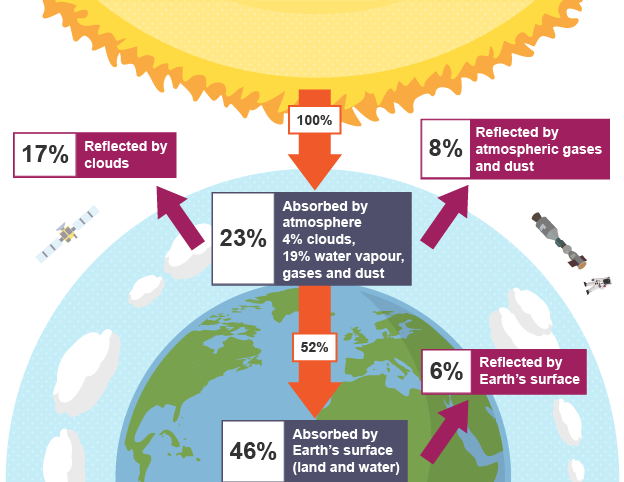
\includegraphics[width=.5\linewidth]{Images/heat_budget.png}
    \caption{The process of insolation within the atmosphere (provided by the BBC)}
\end{figure}

The primary feature of the Earth's thermal energy equilibrium is that there is a net gain of solar radiation in the tropical latitudes and a net loss towards the poles. As evident by figure \ref{energy_balance}, there is a thermal energy deficit between $\pm 35 ^{\circ}$ from the equator and the poles. At these locations, the outgoing radiation exceeds the insolation. Insolation varies wildly depending on the line of latitude at which you are situated; it is as low as approximately $50 J$ at the poles, and peaks at the equator at approximately $275 J$. Terrestrial radiation is less varied, ranging from $120 J$ at the poles to $200 J$ at the equator. 

\begin{figure}[H]
    \centering
    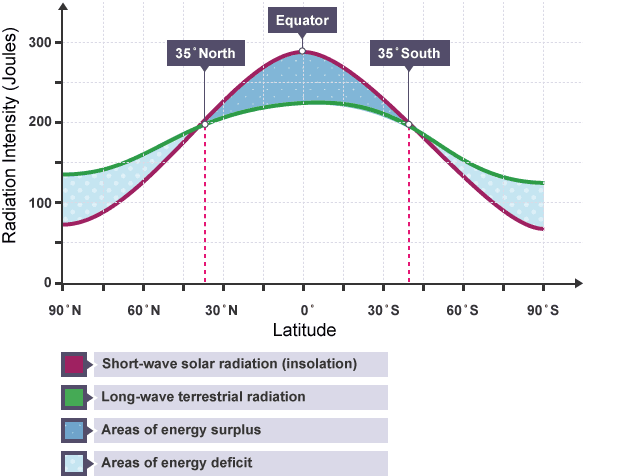
\includegraphics[width=.5\linewidth]{Images/lat_energy_bal.png}
    \caption{Latitude - Radiation Intensity Graph (provided by the BBC)}
    \label{energy_balance}
\end{figure}

Through atmospheric circulation, thermal energy is transferred from areas of low latitude, which have a thermal energy surplus, to areas of high latitude, which have a thermal energy deficit\cite{lat_energy_bal}.

\subsection{Redistrubution of Thermal Energy by Atmospheric Circulation}\label{atmospheric_circulation}
\begin{definition}
Atmospheric circulation is the large-scale movement of air, and together with ocean circulation is the means by which thermal energy is redistributed on the surface of the Earth.
\end{definition}

The atmospheric circulation varies from year to year, but the large-scale structure of its circulation remains fairly constant. A simplified model has been developed in order to explain how the redistrubution of thermal energy from areas of surplus to areas of deficit occurs. It is known as the three-cells model, and can be seen in figure \ref{three_cell}\cite{three_cell}.

\begin{figure}[H]
    \centering
    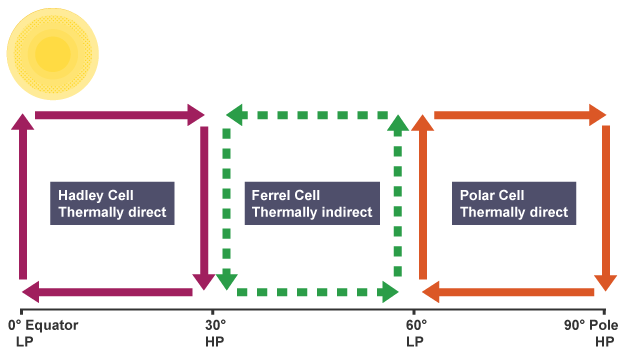
\includegraphics[width=.5\linewidth]{Images/three_cell.png}
    \caption{Three-Cell Atmospheric Circulation Model (provided by the BBC)}
    \label{three_cell}
\end{figure}

Warm air, originating at the equator, ascends creating an area of low pressure, and travels to the 30th parallel, where an area of high pressure is formed. The descended air then travels toward the equator along the surface, replacing the air that rose from the equatorial zone, closing the loop. This is known as the Hadley cell, and it is a closed circulation loop. This atmospheric circulation pattern was developed in an attempt to explain the trade winds, and is considered to be thermally direct; in other words, it exists as a direct consequence of surface temperatures\cite{cells}. As a consequence of this cell, the warmest air does not reach the poles. If atmospheric dynamics were different, however, it is plausible that one large overturning circulation per hemisphere could exist and that wind from the low-latitudes could transport heat to the high-latitudes\cite{hadley_cell}. An eddy is a fluid current whose flow direction differs from that of the general flow.

The Ferrel cell (mid-latitude cell) is located between $30^{\circ}$ and $60^{\circ}$ of latitude. The movement within the Ferrel cell is the reverse of the airflow in the Hadley cell. This cell was the first to account for the westerly winds, more formely known as the `Prevailing Westerlies'. The Ferrell cell is thermally indirect as it is powered by the two other cells. It might be thought of as an eddy created by the Hadley and Polar cells\cite{ferrel}.

The Polar cell is much smaller than the other two cells, and is thermally direct. Similar to the Hadley cell, it operates as a closed circulation loop. As is evident in figure \ref{global_circulation}, cold air sinks at the poles before flowing towards the 60th parallel. Here it is warmed, after which, it rises\cite{cells}. The polar cell, terrain, and Katabatic winds in Antarctica can create very cold conditions at the surface, for instance the lowest temperature recorded on Earth: $183.95 K$ at Vostok Station in Antarctica\cite{polar}.

\begin{figure}[H]
    \centering
    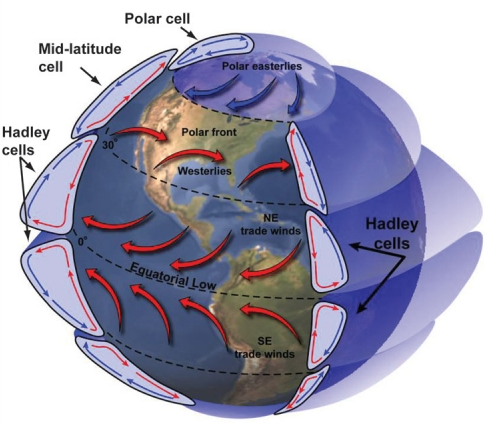
\includegraphics[width=.5\linewidth]{Images/three_cell_globe.png}
    \caption{Idealised Atmospheric Circulation Model (provided by Harvard University)}
    \label{global_circulation}
\end{figure}

The global wind system is created by air blowing from areas of high pressure to areas of low pressure. Winds are affected by the Coriolis effect. In the Northern Hemisphere the Coriolis effect deflects movement to the right and in the Southern Hemisphere it deflects movement to the left.

\section{Ideal Gas Law}\label{ideal}
As mentioned previously, the atmosphere is a continuous stratified fluid with various physical quantities, such as pressure, temperature, and density that characterise its state. Before, one can dive into explaining how one could simulate the dynamics of the atmosphere, it is necessary to briefly touch on the ideal gas equation.

The ideal gas equation is the equation of state for the atmosphere, and is defined as an equation relating temperature, pressure, and specific volume of a system in thermodynamic equilibrium\cite{state_equation}. For most meteorology applications at synoptic scales, it is useful to think of the constituent gases of the atmosphere as ideal gases\cite{ideal_gas}. An ideal gas is an approximation that helps up model and predict the behaviour of real gases. An ideal gas is a hypothetical gas that follows a few rules\cite{iop}: 

\begin{itemize}
    \item The particles of this gas have negligible volume.
    \item The particles of this gas cannot attract, nor repel one another, although they may collide.
    \item Collisions with a surface (i.e. a wall) are elastic.
    \item The motion of the particles in this gas are isotropic. 
\end{itemize}

This idea of an ideal gas forms an equation of state for dry air known as the ideal gas law. This is given by the equation \ref{ideal_gas_law_weird}, or in the form it is more commonly presented in equation \ref{ideal_gas}.

\begin{equation}
    \label{ideal_gas_law_weird}
    p\alpha = RT
\end{equation}

where $\alpha$ is the specific volume.

\begin{equation}
    \label{ideal_gas}
    \Rightarrow p = \rho RT
\end{equation}

It must be noted that there is no gas that is exactly ideal, however, for plenty of gases it is a pretty good approximation. The keen eyed among you may have noticed that it was previously mentioned that stratospheric air is extremely dry. As a result of this, stratospheric air is extremely well described by the ideal gas equation. 

It also must be noted that if the pressure is too large, or the temperature is too low there can be significant deviations from the ideal gas law\cite{ideal_gas}. Considering, however, we are dealing with atmospheric pressure and temperature ranges within the troposphere and the stratosphere, these value extremes will never be reached at any point within them.

\section{Hydrostatic Balance}
\begin{definition}
Hydrostatic Balance describes a balance between vertical pressure gradient and buoyancy forces.
\end{definition}

Another point to examine, before delving into the mathematics of atmospheric dynamics, is to consider a thin horizontal layer of thickness $\Delta z$, as shown in figure \ref{global_circulation}. If we assume that the gas as a whole is at rest, then the layer cannot be gaining or losing momentum. Making note that the pressure is simply the flux of momentum, one can write the vertical momentum budget for the layer as:

\begin{equation}
    p(z) A - p(z + \Delta z) A - A \Delta z \rho g = 0
\end{equation}

\begin{center}
    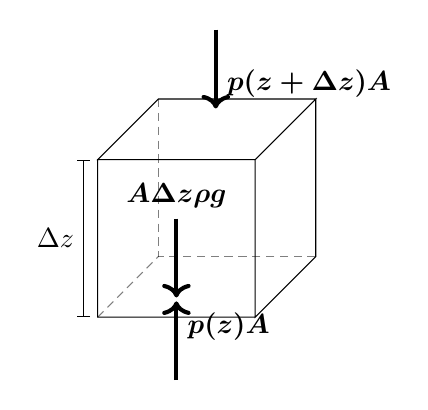
\begin{tikzpicture}[every edge quotes/.append style={auto, text=black}]
        \pgfmathsetmacro{\cubex}{2}
        \pgfmathsetmacro{\cubey}{2}
        \pgfmathsetmacro{\cubez}{2}
        \draw [draw=black, every edge/.append style={draw=black, densely dashed, opacity=.5}]
        (0,0,0) coordinate (o) -- ++(-\cubex,0,0) coordinate (a) -- ++(0,-\cubey,0) coordinate (b) edge coordinate [pos=1] (g) ++(0,0,-\cubez)  -- ++(\cubex,0,0) coordinate (c) -- cycle
        (o) -- ++(0,0,-\cubez) coordinate (d) -- ++(0,-\cubey,0) coordinate (e) edge (g) -- (c) -- cycle
        (o) -- (a) -- ++(0,0,-\cubez) coordinate (f) edge (g) -- (d) -- cycle;
        
        \draw[->, line width=1.5pt](-0.5,1.65) -- (-0.5,0.65) node[anchor=south west]{$\boldsymbol{p(z + \Delta z) A}$};
        \draw[->, line width=1.5pt](-1,-2.80) -- (-1,-1.80) node[anchor=north west]{$\boldsymbol{p(z) A}$};
        \draw[->, line width=1.5pt](-1,-0.75) node[anchor=south]{$\boldsymbol{A \Delta z \rho g}$} -- (-1,-1.75);
        
        \path [every edge/.append style={draw=black, |-|}]
        (b) +(-5pt,0) coordinate (b2) edge ["$\Delta z$"] (b2 |- a);
    \end{tikzpicture}
\end{center}

which can be rearranged as:

\begin{equation}
    \frac{p(z + \Delta z) - p(z)}{\Delta z} = -\rho g
\end{equation}

and in the $\lim_{\Delta z \to 0}$:

\begin{equation}
    \frac{dp}{dz} = -\rho g
\end{equation}

which is the equation of hydrostatic balance. The key assumption of this equation is that the gas is not accelerating in the vertical. It must be noted that strictly speaking the atmosphere is never in precise hydrostatic balance\cite{iop}. At a synoptic scale, however, it is a pretty reasonable approximation. 




\chapter{Simulating Dynamics}\label{3}
\epigraph{``I've got a bad feeling about this"}{Hans Solo}

\section{Geostrophic Wind}\label{geostrophic_wind}
There are a number of forces that can either change the force or direction of wind. Two of the biggest forces of wind vectors are the pressure gradient force and the Coriolis force.

\subsection{Pressure-Gradient Force}
\begin{definition}
The pressure-gradient force is a force acting on air that is due to pressure differences.
\end{definition}

Horizontal variations in pressure create a tendency for movement from higher to lower pressure. The atmosphere, like all systems in nature, is trying to stay at the lowest energy level possible. Therefore, if there is an area of lower pressure nearby, air will freely move from the high pressure area to the low pressure area in order to equalise this energy gradient. To do this, it will attempt to take the shortest distance possible in order to maximise efficiency, which happens to be perpendicular to the isobars\cite{pressuregrad_def}. This phenomenon is described by equation \ref{pressure_grad}, where $P$ is the pressure-gradient force.

\begin{equation}
    \label{pressure_grad}
    P = - \Vec{\nabla} p
\end{equation}

The negative sign at the beginning of the equation designates that we move from high to low across the pressure gradient. The greater the difference in pressure between the two locations, the greater the pressure gradient. A stronger pressure-gradient force usually correlates to a stronger wind vector. It must be noted that the pressure-gradient force is only one component of the forces acting on the actual wind, though, so, air does not normally flow perpendicular to the isobars\cite{pressure_grad}.

\subsection{Coriolis Force}\label{f_section}
\begin{definition}
The Coriolis force is an inertial force that acts on objects that are in motion within a frame of reference that rotates with respect to an inertial frame.
\end{definition}

The Coriolis force ultimately results in the diversion of the wind's direction within the atmosphere due to the Earth's rotation. The Earth is spinning in a prograde direction. The Earth is a elongated spheroid, however, to a reasonable good approximation, it can be considered to be a sphere. Due to this fact, all points on the surface of the Earth are travelling at the same angular velocity. As a consequence, however, a point near the equator must have a higher linear velocity, as it must travel a larger distance than a point near the poles. When an object moves either closer or further from the equator its original momentum is preserved, giving the path a diversion off its original course\cite{corioliseffect_def}. If the wind is travelling in accordance with the pressure-gradient force, the wind will be deflected off its original course by the Coriolis force. It must be noted that there isn't a Coriolis force at the equator, however, it increases with intensity as one approaches the poles. The Coriolis force is described by equation \ref{coriolis_force}.

\begin{equation}
    \label{coriolis_force}
    F = \rho U f_0
\end{equation}

where $f_0$ is the Coriolis parameter, and is given by equation \ref{f}.

\begin{equation}
    \label{f}
    f_0 = 2 \Omega \sin{\phi}
\end{equation}

One can therefore deduce that the higher the latitude, the higher the Coriolis force. Also, the Coriolis force only acts on air that is already set into motion. The Coriolis force will not set wind into motion, but will only deflect the direction of wind that is already moving. Therefore, it follows that the faster that air is moving, the stronger it is affected by the Coriolis force\cite{coriolis_effect}. 

Equation \ref{f} is known as the f-plane approximation, which can be visualised as a tangent plane touching the surface of the sphere at this latitude. The beta plane approximation is, however, utilised in the quasi-geostrophic theory, which ignores the variation of $f$ with latitude. In this approximation, $f$ is set to vary linearly in space and a value of $f$ appropriate for a particular latitude is used throughout the domain. The equation describing the beta plane approximation is as follows:

\begin{equation}
    f = f_0 + \beta y
\end{equation}

The advantage of the beta plane approximation over more accurate formulations is that it does not contribute nonlinear terms to the dynamical equations\cite{beta_approx}. $\beta$ in the above equation is the Rossby number, which is discussed in the following section\cite{rossby_number}.

\subsection{Geostrophic Balance}\label{balance}
\begin{definition}
Geostrophic Balance is an exact balance between the Coriolis force and the pressure-gradient force.
\end{definition}

This balance seldom holds true in nature. This concept, however, will lead to the development of a theoretical wind, known as geostrophic wind. First and foremost, lets introduce the horizontal momentum equations.

\begin{equation}
    \frac{Du}{Dt} = -\frac{1}{\rho}\frac{\partial p}{\partial x} + f v
\end{equation}

\begin{equation}
    \frac{Dv}{Dt} = -\frac{1}{\rho}\frac{\partial p}{\partial y} - f  u
\end{equation}

Assuming geostrophic balance, the system is stationary and the first two equations become:  

\begin{equation}
    u = -\frac{1}{\rho f} \frac{\partial p}{\partial y}
\end{equation}

\begin{equation}
    v = \frac{1}{\rho f} \frac{\partial p}{\partial x}
\end{equation}

\begin{definition}
Geostrophic Wind is the wind that flows parallel to height contours or isobars resulting from an exact balance between the Coriolis force and the pressure-gradient force.
\end{definition}

The geostrophic wind vector can also be expressed in terms of the gradient of the geopotential on a surface of constant pressure. This is extremely useful as it also for the calculation of geostrophic wind through the utilisation of geopotential height. It also allows for the calculation of geostrophic wind in an isobaric co-ordinate system. Therefore, the above equations are rewritten as follows:

\begin{equation}
    u_g = -\frac{g}{f} \frac{\partial \Phi}{\partial y}
    \label{u_g}
\end{equation}

\begin{equation}
    v_g = \frac{g}{f} \frac{\partial \Phi}{\partial x}
    \label{v_g}
\end{equation}

Any spatial derivatives within this equation are replaced by a central difference approximation of the derivatives, which results in:

\begin{equation}
    u_g = -\frac{g}{f} \frac{\Delta \Phi}{2 \Delta y}
\end{equation}

\begin{equation}
    v_g = \frac{g}{f} \frac{\Delta \Phi}{2 \Delta x}
\end{equation}

For the geostrophic flow concept to work, the wind must not be changing speed (is unaccelerated or the acceleration is almost zero). The question remains whether geostrophic wind is a good approximation for the actual wind. The tendency for wind to be accelerated can be measured at various scales of circulation. Meanwhile, the Coriolis acceleration is only related to the speed of the object and its latitude. Thus, as the flow  approaches geostrophic the smaller the actual acceleration is relative to the Coriolis acceleration\cite{geo_wind}.

\begin{definition}
Rossby Number is the ratio of the total acceleration to the Coriolis acceleration.
\end{definition}

If the Rossby number is small (less than one), the geostrophic wind is a reasonably good approximation for geostrophic wind, neglecting the force of friction in this assumption. From table 3.1, generally the geostrophic wind is a good approximation if it is determined at a synoptic scale\cite{geo_wind}. 

\hfill

\begin{center}
\begin{tabular}{|c|c|c|} 
 \hline
 Scale of Circulation & Rossby Number & Yes / No \\
 \hline
 10,000 km & 0.01 & Yes \\
 \hline
 1,000 km & 0.1 & Yes \\
 \hline
 100 km & 1.0 & Not Really \\
 \hline
 10 km & 3.0 & No \\
 \hline
 1 km & 4.0 & No \\
 \hline
\end{tabular}\par
\bigskip
Table 3.1.: Is geostrophic wind a good approximation for the real wind?
\end{center}

\section{Pressure Thickness}\label{pressure_thickness}
\begin{definition}
Pressure Thickness is the measurement of the distance (in metres) between any two constant pressure surfaces.
\end{definition}

\begin{figure}[H]
    \centering
    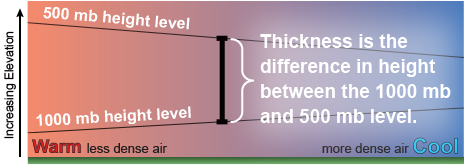
\includegraphics[width=.8\linewidth]{Images/thickness_def.png}
    \caption{Pressure Thickness Definition (provided by the NWS of the USA)}
    \label{thickness_def}
\end{figure}

One of the most common thickness charts used in meteorology is the 1000-500 hPa thickness, and for the purposes of this project, it will be the sole interest. This is the distance between the elevation of the 1,000 hPa and 500 hPa levels. Typically, the 1,000 hPa surface is used to represent sea level but this is just a generalisation. On pressure charts, the last digit (zero) of a thickness value is typically truncated. So, a 1000-500 thickness value of 570 means the distance between the two surfaces is 5,700 metres. The 1000-500 hPa thickness value of 540 is traditionally used to determine rain versus snow. If precipitation is predicted poleward of this 540-thickness line (if the thickness value is less than 540), it is expected that it will be snow. If precipitation is predicted on the equator side of this line (if the thickness value is greater than 540), then it is expected that the precipitation will be in a liquid form. The reason one is able to make such an expectation is due to the fact that the 540-thickness line closely follows the surface freezing temperature of 273 K\cite{thickness}.

\begin{figure}[H]
    \centering
    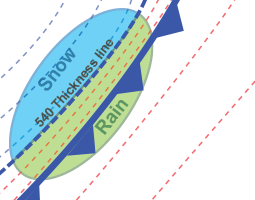
\includegraphics[width=.4\linewidth]{Images/rainsnow_line.png}
    \caption{Rain/Snow Line (provided by the NWS of the USA)}
    \label{rainsnow_line}
\end{figure}

To determine the pressure thickness between two constant pressure surfaces, the Hypsometric equation is utilised and as shown in equation \ref{hypsometric}. 

\begin{definition}
The hypsometric equation relates an atmospheric pressure ratio to the equivalent thickness of an atmospheric layer considering the layer mean of virtual temperature, gravity, and occasionally wind. It is derived from the hydrostatic equation and the ideal gas law.
\end{definition}

\begin{equation}
    \label{hypsometric}
    h = \Phi_2 - \Phi_1 = \frac{R \bar{T_v}}{g} \ln{\frac{p_1}{p_2}}
\end{equation}

\section{Precipitable Water}
\begin{definition}
Precipitable Water is the total atmospheric water vapour contained in a vertical column of unit cross-sectional area extending between any two specified pressure levels.
\end{definition}

Based on the definition, precipitable water can be described mathematically as being:

\begin{equation}
    \label{pwv_1}
    W = \int_{0}^{z} \rho_v dz
\end{equation}

where $\rho_v$ is the density of water vapour, and where $\rho_v$ is defined as:

\begin{equation}
    \rho_v = \frac{\texttt{mass of vapour}}{\texttt{unit volume}}
\end{equation}

Following which, the hydrostatic equation can be applied to equation \ref{pwv_1} in order to replace $dz$ with $dp$. The reason for doing this is that atmospheric pressure is extremely easier to measure, with devices such as weather balloons being readily available.

\begin{equation}
    \label{pwv_derive}
    W = -\int_{p_1}^{p_2} \frac{\rho_v}{\rho g} dp
\end{equation}

Where $p_1$ and $p_2$ are constant pressure surfaces, and where $p_1 > p_2$. Substituting in the definition of density, $\rho_v = \frac{m_v}{V}; \rho = \frac{m_{air}}{V}$, into equation \ref{pwv_derive} results in:

\begin{equation}
    W = -\int_{p_1}^{p_2} \frac{1}{g} \frac{m_v V}{m_{air} V} dp
\end{equation}

\begin{equation}
    \Rightarrow W = - \frac{1}{g} \int_{p_1}^{p_2} \frac{m_v}{m_{air}} dp
\end{equation}

The integration term in this particular equation is the definition for the specific humidity, with the units of measurement being $\frac{kg}{kg}$. The specific humidity can be approximated by the mixing ratio, with an error typically around 4 \%\cite{pwv_def}.

\begin{definition}
Mixing Ratio is the ratio of the mass of a variable atmospheric constituent to the mass of dry air.
\end{definition}

\begin{equation}
    \label{pwv_derive_fin}
    \therefore W = -\frac{1}{g} \int_{p_1}^{p_2} m dp
\end{equation}

The units as given by the equation are $\frac{kg}{m^2}$ (dimensionless), but, the preferred unit of measurement for rainfall is $mm$. The conversion between the two units of measurements is one to one ($1 \frac{kg}{m^2} = 1 mm$) In actual rainstorms, particularly thunderstorms, amounts of rain very often exceed the total precipitable water of the overlying atmosphere. This results from the action of convergence that brings into the rainstorm the water vapour from a surrounding area that is often quite large. Nevertheless, there is general correlation between precipitation amounts in given storms and the precipitable water of the air masses involved in those storms\cite{problems_with_pwv}.

For the purposes of numerically calculating the precipitable water for a given column of air, equation \ref{pwv_derive_fin} is commonly rewritten as the following:

\begin{equation}
    \label{pwv}
    W = -\frac{1}{\rho g} \int_{p_1}^{p_2} \frac{0.622 e}{p - e} dp
\end{equation}

\begin{definition}
Vapour Pressure is the pressure exerted by a vapour when the vapour is in equilibrium with the liquid or solid form, or both, of the same substance. In meteorology, vapour pressure is used almost exclusively to denote the partial pressure of water vapour in the atmosphere.
\end{definition}

Considering vapor pressure is not one of the three prognostic variables defined in section \ref{noaa_initial_conditions}, it is therefore necessary to express vapor pressure in terms of the already defined variables. This can be done through the utilisation of temperature and relative humidity. First, one must determine the saturated vapour pressure. This can be done using the following equation\cite{balton}:

\begin{equation}
    e_s = 6.112 \exp(\frac{17.67 T}{T + 243.5})
\end{equation}

After which, the vapor pressure can be calculated as follows:

\begin{equation}
    e = \frac{e_{s} r}{100}
    \label{vapor_pressure_eq}
\end{equation}

In wet periods, the precipitable water is particularly close to the saturated precipitable water. In situations when the precipitable water is close to the saturated precipitable water, the precipitable water changes very little over the day. Saturated precipitable water also makes calculations a whole lot simpler, as specific humidity data is rather difficult to come by.

In regards to the numerical calculation of the precipitable water, the SciPy method, scipy.integrate.quad, is utilised in order to determine the definite integral in equation \ref{pwv}. This method integrates the function using a technique from the Fortran library, QUADPACK\cite{scipy_integrate}. 

\section{Virtual Temperature}\label{virtual_section}
The virtual temperature is the temperature at which dry air would have the same density as the moist air, at a given pressure. In other words, two air samples with the same virtual temperature have the same density, regardless of their actual temperature or relative humidity. Because water vapor is less dense than dry air and warm air is less dense than cool air, the virtual temperature is always greater than or equal to the actual temperature. 

In relation to this project, the virtual temperature will be extremely useful as it will allow for the calculation of the evolution of relative humidity through the utilisation of the thermodynamic advection equation (which is discussed in section \ref{advection_equation}). This is due to the fact that virtual temperature can be expressed in terms of vapor pressure, which can be converted into relative humidity.  This can be seen as follows:

\begin{equation}
    T_v = \frac{T}{1 - \frac{0.378 e}{p}}
\end{equation}

The equation becomes the following, by substituting equation \ref{vapor_pressure_eq} in and rearranging for relative humidity:

\begin{equation}
    r = \frac{100 (p T_v - p T)}{0.378 e_s T_v}
\end{equation}

\section{Quasi-Geostrophic Theory}
\subsection{Introduction}
From numerical weather prediction, the public desires information pertaining to the temperature, wind speed, wind direction and humidity in their area up to 7 days in advance. This information is largely a function of evolving synoptic weather patterns (for example, fronts and jet streams). The basic idea of quasi-geostrophic theory is that it reveals how hydrostatic balance and geostrophic balance constrain and simply atmospheric dynamics, but, in a realistic manner. It provides a framework by which an understanding of, and an ability to diagnose, the evolution of a three dimensional synoptic-scale weather system. It achieves this by providing insights into how mass fields and momentum fields interact to create vertical circulations that result in realistic synoptic-scale weather patterns.

\subsection{Thermodynamic Equation}\label{advection_equation}
To begin with, the thermodynamic equation will be the primary focus. The first thing to examine in the thermodynamic equation is advection. As mentioned previously, advection is a horizontal transfer of mass, heat, or other property. Accordingly, winds that blow across Earth's surface represent advectional movements of air. 

Differential temperatures drive the mass movement of air seeking equilibrium. Advective winds move from areas of higher temperature toward areas of lower temperature. In contrast, convection, the vertical movement of mass or transfer of heat, manifests itself as air currents. Accordingly, winds are a result of advection, while air currents are a result of convection. In the atmosphere, advection is the sole process of horizontal transfer of mass. In contrast, vertical transfer occurs via conduction, convection, and radiation.

The magnitude of heat transference depends on the rate of heat transport, and flux in turn relates the transfer of heat energy in terms of area and time\cite{advection}. Advection can be represented in vector notation by:

\begin{equation}
    \frac{\partial T}{\partial t} + \Vec{v} \cdot \nabla_p T = 0
\end{equation}

The del operator ($\nabla_p$) will be expanded into its components as shown in equation \ref{del_operator}. The reason for doing so is that it makes the equation easier to work with down the line.

\begin{equation}
    \Rightarrow \frac{\partial T}{\partial t} + \begin{bmatrix} \Vec{v}_x \\ \Vec{v}_y \\ \Vec{v}_p \end{bmatrix} \cdot \begin{bmatrix} \frac{\partial}{\partial x} \hat{i} \\ \frac{\partial}{\partial y} \hat{j} \\ \frac{\partial}{\partial p} \hat{k} \end{bmatrix} T
    \label{del_operator} = 0
\end{equation}

Taking the dot product results in the following:

\begin{equation}
     \frac{\partial T}{\partial t} = - (\Vec{v_{x}} \frac{\partial}{\partial x} \hat{i} + \Vec{v_{y}} \frac{\partial}{\partial y} \hat{j} + \Vec{v_{p}} \frac{\partial}{\partial p} \hat{k}) T
\end{equation}

Expanding the brackets results in:

\begin{equation}
     \frac{\partial T}{\partial t} = -\Vec{v_{x}} \frac{\partial T_{x}}{\partial x} - \Vec{v_{y}} \frac{\partial T_{y}}{\partial y} - \Vec{v_{p}} \frac{\partial T_{p}}{\partial p} 
\end{equation}

\begin{equation}
    \Rightarrow \frac{\partial T}{\partial t} = -u \frac{\partial T}{\partial x} - v \frac{\partial T}{\partial y} - \omega \frac{\partial T}{\partial p}
\end{equation}

The terms on the RHS are due to advection within the atmosphere. Each $T$ is actually different and related to its respective plane. This is divided by the distance between grid points to get the change in temperature with the change in distance. When multiplied by the wind velocity on that plane, the units $K m^{-1}$ and $m s^{-1}$ give $K s^{-1}$. The sum of all the changes in temperature due to motions in the $x$, $y$, and $p$ directions give the total change in temperature with time\cite{primitive_equations}.

This is the almost complete version of the thermodynamic equation, however, it is also necessary to add an additional term for vertical transfer, hence, the above equation becomes the following:

\begin{equation}
    \Rightarrow \frac{\partial T}{\partial t} = -u \frac{\partial T}{\partial x} - v \frac{\partial T}{\partial y} - \omega \frac{\partial T}{\partial p} + \omega \frac{R T}{p c_p}
\end{equation}

It is then possible to combine the two terms containing vertical motion resulting in:

\begin{equation}
    \Rightarrow \frac{\partial T}{\partial t} = -u \frac{\partial T}{\partial x} - v \frac{\partial T}{\partial y} + \omega \sigma \frac{p}{R}
    \label{analytic_temp_final}
\end{equation}

This equation describes temperature changing at a particular location and height is a function of temperature advection and vertical motion. Warm advection causes a temperature increase. Ascent causes adiabatic cooling and a temperature decrease, while descent produces adiabatic heating. These two terms often oppose each other. 

\begin{definition}
Adiabatic cooling is the process of reducing heat through a change in air pressure caused by volume expansion.
\end{definition}

For example, strong warm advection at a level causes local warming, but often ascent as well. The ascent leads to adiabatic cooling opposing the warming due to warm advection. Given strong ascent, this can contribute to isotherms (lines on a weather showing areas of equal temperature) remaining steady or even sinking southward in the face of warm advection, which may be very important for heavy precipitation production. Models can show this process, which likely will be accompanied by areas of strong model upward motion. In borderline precipitation phase change situations, the absence of strong ascent can result in, for example, drizzle. However, if a burst of vertical motion develops in this area, strong adiabatic cooling can temporary cause a phase change to snow, with precipitation diminishing and changing back to liquid once the enhanced ascent zone moves away\cite{describe_quasi}.

Discretizing equation \ref{analytic_temp_final}, by the method described in section \ref{fdm_section} results in:

\begin{equation}
    \frac{T^{n + 1}_{x, y, z} - T^{n - 1}_{x, y, z}}{2 \Delta t} = -u \frac{T^{n}_{x+1, y, z} - T^{n}_{x-1, y, z}}{2 \Delta x} - v \frac{T^{n}_{x, y+1, z} - T^{n}_{x, y-1, z}}{2 \Delta y} + \omega \sigma \frac{p}{R}
\end{equation}

Multiplying both the LHS and the RHS by $2 \Delta t$ in order to isolate the change in temperature with respect to time term results in the following:

\begin{equation}
     T^{n + 1}_{x, y, z} - T^{n - 1}_{x, y, z} = - u \frac{2 \Delta t}{2 \Delta x} (T^{n}_{x+1, y, z} - T^{n}_{x-1, y, z}) - v \frac{2 \Delta t}{2 \Delta y} (T^{n}_{x, y+1, z} - T^{n}_{x, y-1, z}) + \omega \sigma \frac{p}{R}
\end{equation}

Rearranging the equation in order to isolate the $T^{n + 1}_{x, y, z}$ term: 

\begin{equation}
     T^{n + 1}_{x, y, z} = T^{n - 1}_{x, y, z} - u \frac{2 \Delta t}{2 \Delta x} (T^{n}_{x+1, y, z} - T^{n}_{x-1, y, z}) - v \frac{2 \Delta t}{2 \Delta y} (T^{n}_{x, y+1, z} - T^{n}_{x, y-1, z}) + \omega \sigma \frac{p}{R}
\end{equation}

This discretized equation will allow for the calculation of the evolution of temperature and virtual temperature. Hence, this will also allow for the calculation of the evolution of relative humidity as described in section \ref{virtual_section}.

\subsection{Height Tendency Equation}
In order to predict system evolution, it is necessary to examine changes in the local height field. Therefore, the goal is to develop a single prognostic equation for geopotential height. Although the vertical velocity plays an essential role in the dynamics, the evolution of the geostrophic circulation can be determined without explicitly determining the distribution of the vertical velocity\cite{eq_describe}. To do this, it is necessary to begin with the definition of geostrophic relative vorticity:

\begin{equation}
    \zeta_g = \frac{\partial v_g}{\partial y} - \frac{\partial u_g}{\partial x}
    \label{zeta}
\end{equation}

The relative vorticity is the vorticity (a measure of the local rotation of a fluid) relative to the Earth induced by the air velocity field. In the case of geostrophic relative vorticity, the air velocity field would be the geostrophic wind. This air velocity field is modelled as a two-dimensional flow parallel to the ground, so that the relative vorticity vector is generally a scalar rotation quantity perpendicular to the ground. Vorticity is positive, when looking down on the Earth and when the wind is turning counterclockwise\cite{vorticity}. The following can be shown, by, substituting equations \ref{u_g} and \ref{v_g} into equation \ref{zeta}:

\begin{equation}
    \zeta_g = \frac{1}{f_0} \nabla^{2}_p \varphi      
\end{equation}

\begin{definition}
Geopotential is the potential of the Earth's gravity field. For convenience it is often defined as the negative of the potential energy per unit mass, so that the gravity vector is obtained as the gradient of this potential, without the negation.
\end{definition}

Redefining the hydrostatic equation in section \ref{hydro_balance} in isobaric coordinates results in the following:

\begin{equation}
    g \frac{\partial \Phi}{\partial p} = - \frac{R T}{p}
\end{equation}

Using the definition of geopotential $\varphi = g \Phi$, it is possible to rearrange the above equation in terms of temperature:

\begin{equation}
    T = - \frac{p}{R} \frac{\partial \varphi}{\partial p}    
\end{equation}

It is now possible to define local changes in vorticity and temperature in terms of the local height tendency on constant pressure surfaces:

\begin{equation}
    \frac{\partial \zeta_g}{\partial t} = \frac{\partial}{\partial t} (\frac{1}{f_0} \nabla^{2}_p \varphi) = \frac{1}{f_0} \nabla^{2}_p \frac{\partial \varphi}{\partial t}
\end{equation}

\begin{equation}
    \frac{\partial T}{\partial t} = \frac{\partial}{\partial t} (- \frac{p}{R} \frac{\partial \varphi}{\partial p}) = - \frac{p}{R} \frac{\partial (\frac{\partial \varphi)}{\partial t}}{\partial p} 
\end{equation}

For compactness, $\frac{\partial \varphi}{\partial t}$ will be defined as $\varphi_t$, therefore, the above equations become:

\begin{equation}
    \frac{\partial \zeta_g}{\partial t} = \frac{1}{f_0} \nabla^{2}_p \varphi_t
    \label{zeta_relationship}
\end{equation}

\begin{equation}
    \frac{\partial T}{\partial t} = - \frac{p}{R} \frac{\partial \varphi_t}{\partial p} 
\end{equation}

These two relationships are very powerful and will be used to physically interpret the terms in the height tendency. It is now possible to substitute the new relationship for temperature into the thermodynamic equation, which results in:

\begin{equation}
    - \frac{p}{R} \frac{\partial \varphi_t}{\partial p} = -u \frac{\partial T}{\partial x} - v \frac{\partial T}{\partial y} + \omega \sigma \frac{p}{R}
\end{equation}

It is also possible to substitute the vorticity relationship into something known as the quasi-geostrophic vorticity equation. This equation is mathematically defined as the following:

\begin{equation}
    \frac{\partial \zeta_g}{\partial t} = -u \frac{\partial \zeta_g}{\partial x} - v \frac{\partial \zeta_g}{\partial y} + f_0 \frac{\partial \omega}{\partial p} - \beta v_g
\end{equation}

This equation states that vorticity changes at a location are due to vorticity advection and vertical divergence. Positive vorticity advection causes geostrophic relative vorticity to increase with time. A vertical divergence results in a vorticity increase. It is, therefore, possible to see how positive vorticity advection and negative vorticity advection affect vorticity at a point\cite{describe_quasi}. Therefore, substituting the relationship established in equation \ref{zeta_relationship} into the quasi-geostrophic vorticity equation results in:

\begin{equation}
    \frac{1}{f_0} \nabla^{2}_p \varphi_t = -u \frac{\partial \zeta_g}{\partial x} - v \frac{\partial \zeta_g}{\partial y} + f_0 \frac{\partial \omega}{\partial p} - \beta v_g
\end{equation}

It is now possible to derive a single prognostic equation for geopotential (diagnostic equation for $\varphi_t$)\cite{quasi_geo}. To do this, it is necessary to eliminate the vertical motion from both equations by:

\begin{enumerate}
    \item Apply the operator $-\frac{f^{2}_0}{\sigma} \frac{\partial}{\partial p} (\frac{R}{p})$ to the thermodynamic equation.
    \item Multiply the quasi-geostrophic vorticity equation by $f_0$.
    \item Add the results of the two proceeding steps.
\end{enumerate}

After a lot of tedious mathematics, the following diagnostic equation is obtained:

\begin{equation}
    (\nabla^2_p + \frac{f^2_0}{\sigma} \frac{\partial^2}{\partial p^2}) \varphi_t = - f_0 \Vec{v_g} \cdot \nabla_p (\zeta_g + f) - \frac{f^2_0}{\sigma} \frac{\partial}{\partial p} (\frac{R}{p} (-\Vec{v_g} \cdot \nabla_p T))
    \label{complex_qg}
\end{equation}

To obtain an actual value for $\varphi_t$, it would be necessary to compute the forcing terms from the three-dimensional wind and temperature fields, and then invert the operator on the LHS using appropriate boundary conditions. This is not a simple task, and forecasters never do this. Rather, for synoptic-scale atmospheric waves, this term is proportional to $-\varphi_t$. This term can be as the local geopotential tendency\cite{quasi_geo}. Therefore, equation \ref{complex_qg} becomes the following:

\begin{equation}
    - \varphi_t = - f_0 \Vec{v_g} \cdot \nabla_p (\zeta_g + f) - \frac{f^2_0}{\sigma} \frac{\partial}{\partial p} (\frac{R}{p} (-\Vec{v_g} \cdot \nabla_p T))
\end{equation}

\begin{equation}
    \Rightarrow \varphi_t = f_0 \Vec{v_g} \cdot \nabla_p (\zeta_g + f) + \frac{f^2_0}{\sigma} \frac{\partial}{\partial p} (\frac{R}{p} (-\Vec{v_g} \cdot \nabla_p T))
\end{equation}

\begin{equation}
    \Rightarrow \frac{\partial \varphi}{\partial t} = \underbrace{f_0 \Vec{v_g} \cdot \nabla_p (\zeta_g + f)}_{\texttt{Term A}} + \underbrace{\frac{f^2_0}{\sigma} \frac{\partial}{\partial p} (\frac{R}{p} (-\Vec{v_g} \cdot \nabla_p T))}_{\texttt{Term B}}
    \label{complex_qg_proportional}
\end{equation}

Term A is proportional to the advection of absolute vorticity. For the upper troposphere it is usually the dominant term.
For short waves we have seen that the relative vorticity advection dominates the planetary vorticity advection. Term B is proportional to minus
the rate of change of temperature advection with respect to pressure. It is therefore related to plus the rate of change of temperature advection with respect to height. This is called the differential temperature advection. The magnitude of the temperature advection tends to be largest in the lower troposphere\cite{describe_quasi}.

In order to allow for numerical computation, it is necessary to discretize (the discretization process is described in great depth in section \ref{fdm_section}). Based on this, term A becomes the following:

\begin{equation}
    A = f_0 \Vec{v_g} \cdot \nabla_p (\zeta_g + f)
\end{equation}

\begin{equation}
    \Rightarrow A = f_0 (u_g \frac{\partial (\zeta_g + f)}{\partial x} + v_g \frac{\partial (\zeta_g + f)}{\partial y})
\end{equation}

\begin{equation}
    \Rightarrow A = f_0 u_g \frac{\partial (\zeta_g + f)}{\partial x} + f_0 v_g \frac{\partial (\zeta_g + f)}{\partial y}
\end{equation}

\begin{equation}
    \Rightarrow A = f_0 u_g \frac{(\zeta_g + f)^{n}_{x+1, y, z} - (\zeta_g + f)^{n}_{x-1, y, z}}{2 \Delta x} + f_0 v_g \frac{(\zeta_g + f)^{n}_{x, y+1, z} - (\zeta_g + f)^{n}_{x, y-1, z}}{2 \Delta y}
\end{equation}

By a similar process, term B becomes the following:

\begin{equation}
    B = \frac{f^2_0}{\sigma} \frac{\partial}{\partial p} (\frac{R}{p} (-u_g \frac{\partial T}{\partial x} - v_g \frac{\partial T}{\partial y}))
\end{equation}

\begin{equation}
    \Rightarrow B = \frac{f^2_0}{\sigma} \frac{1}{ 2 \Delta p} (\frac{R}{p} (-u_g \frac{T^{n}_{x+1, y, z} - T^{n}_{x-1, y, z}}{2 \Delta x} - v_g \frac{T^{n}_{x, y+1, z} - T^{n}_{x, y-1, z}}{2 \Delta y})
\end{equation}

Substituting these discretized terms into equation \ref{complex_qg_proportional}, it becomes the following after following a similar discretization process:

\begin{equation}
    \frac{\partial \varphi}{\partial t} = A + B
\end{equation}

\begin{equation}
    \Rightarrow \frac{\varphi^{n+1}_{x, y, z} - \varphi^{n-1}_{x, y, z}}{2 \Delta t} = A + B
\end{equation}

\begin{equation}
    \Rightarrow \varphi^{n+1}_{x, y, z} - \varphi^{n-1}_{x, y, z} = 2 \Delta t(A + B)
\end{equation}

\begin{equation}
    \Rightarrow \varphi^{n+1}_{x, y, z} = \varphi^{n-1}_{x, y, z} + 2 \Delta t(A + B)
\end{equation}

This discretized equation now allows for the computation of the evolution of geopotential. By using the definition of geopotential $\varphi = g \Phi$, it is possible to determine the geopotential height by rearranging the equation to $\Phi = \frac{\varphi}{g}$, which in turns allows for the computation of the geostrophic wind as described in section \ref{geostrophic_wind}\cite{quasi_geo}.


\chapter{Implementation Details}\label{4}
\epigraph{``Curious that we spend more time congratulating people who have succeeded than encouraging people who have not."}{Neil deGrasse Tyson}

\section{Open Source Software}
As mentioned previously, and to the author's knowledge, there is no open source software currently available that can numerically simulate the dynamics of the atmosphere. But, what is open source software, what are its advantages, and why is it important?

\begin{definition}
Open Source Software is software with source code that anyone can inspect, modify, and enhance. 
\end{definition}

Source code is the code that computer programmers use to modify, and change how a piece of software functions\cite{what_oss}. Programmers with access to the source code can improve that program by adding features to it, fixing bugs, or by improving the documentation of the surrounding source code. 

According to Tom Macaulay\cite{advantages}, the open source development of software has a number of advantages over the traditional development of proprietary software, including but not limited to:

\begin{itemize}
    \item Lower costs.
    \item Extensive customisation.
    \item Higher quality software.
    \item Greater security.
    \item Regular updates.
    \item Quick fixes.
\end{itemize}

If an atmospheric dynamics simulator became available to the open source community, it could lead to a low cost, and high quality simulator ultimately being produced. If such an event occurs, it could, theoretically, vastly enhance existing weather predicting software, and could lead to a further dramatic decline in deaths from weather related phenomena. This project is an attempt to kick start such a future.

Everything related to this project, from the source code of the simulator to this very paper, can be accessed at the organisation known as `AMSIMP' on the open source platform known as GitHub. This can be accessed at \url{https://github.com/amsimp}. 

\begin{figure}[H]
    \centering
    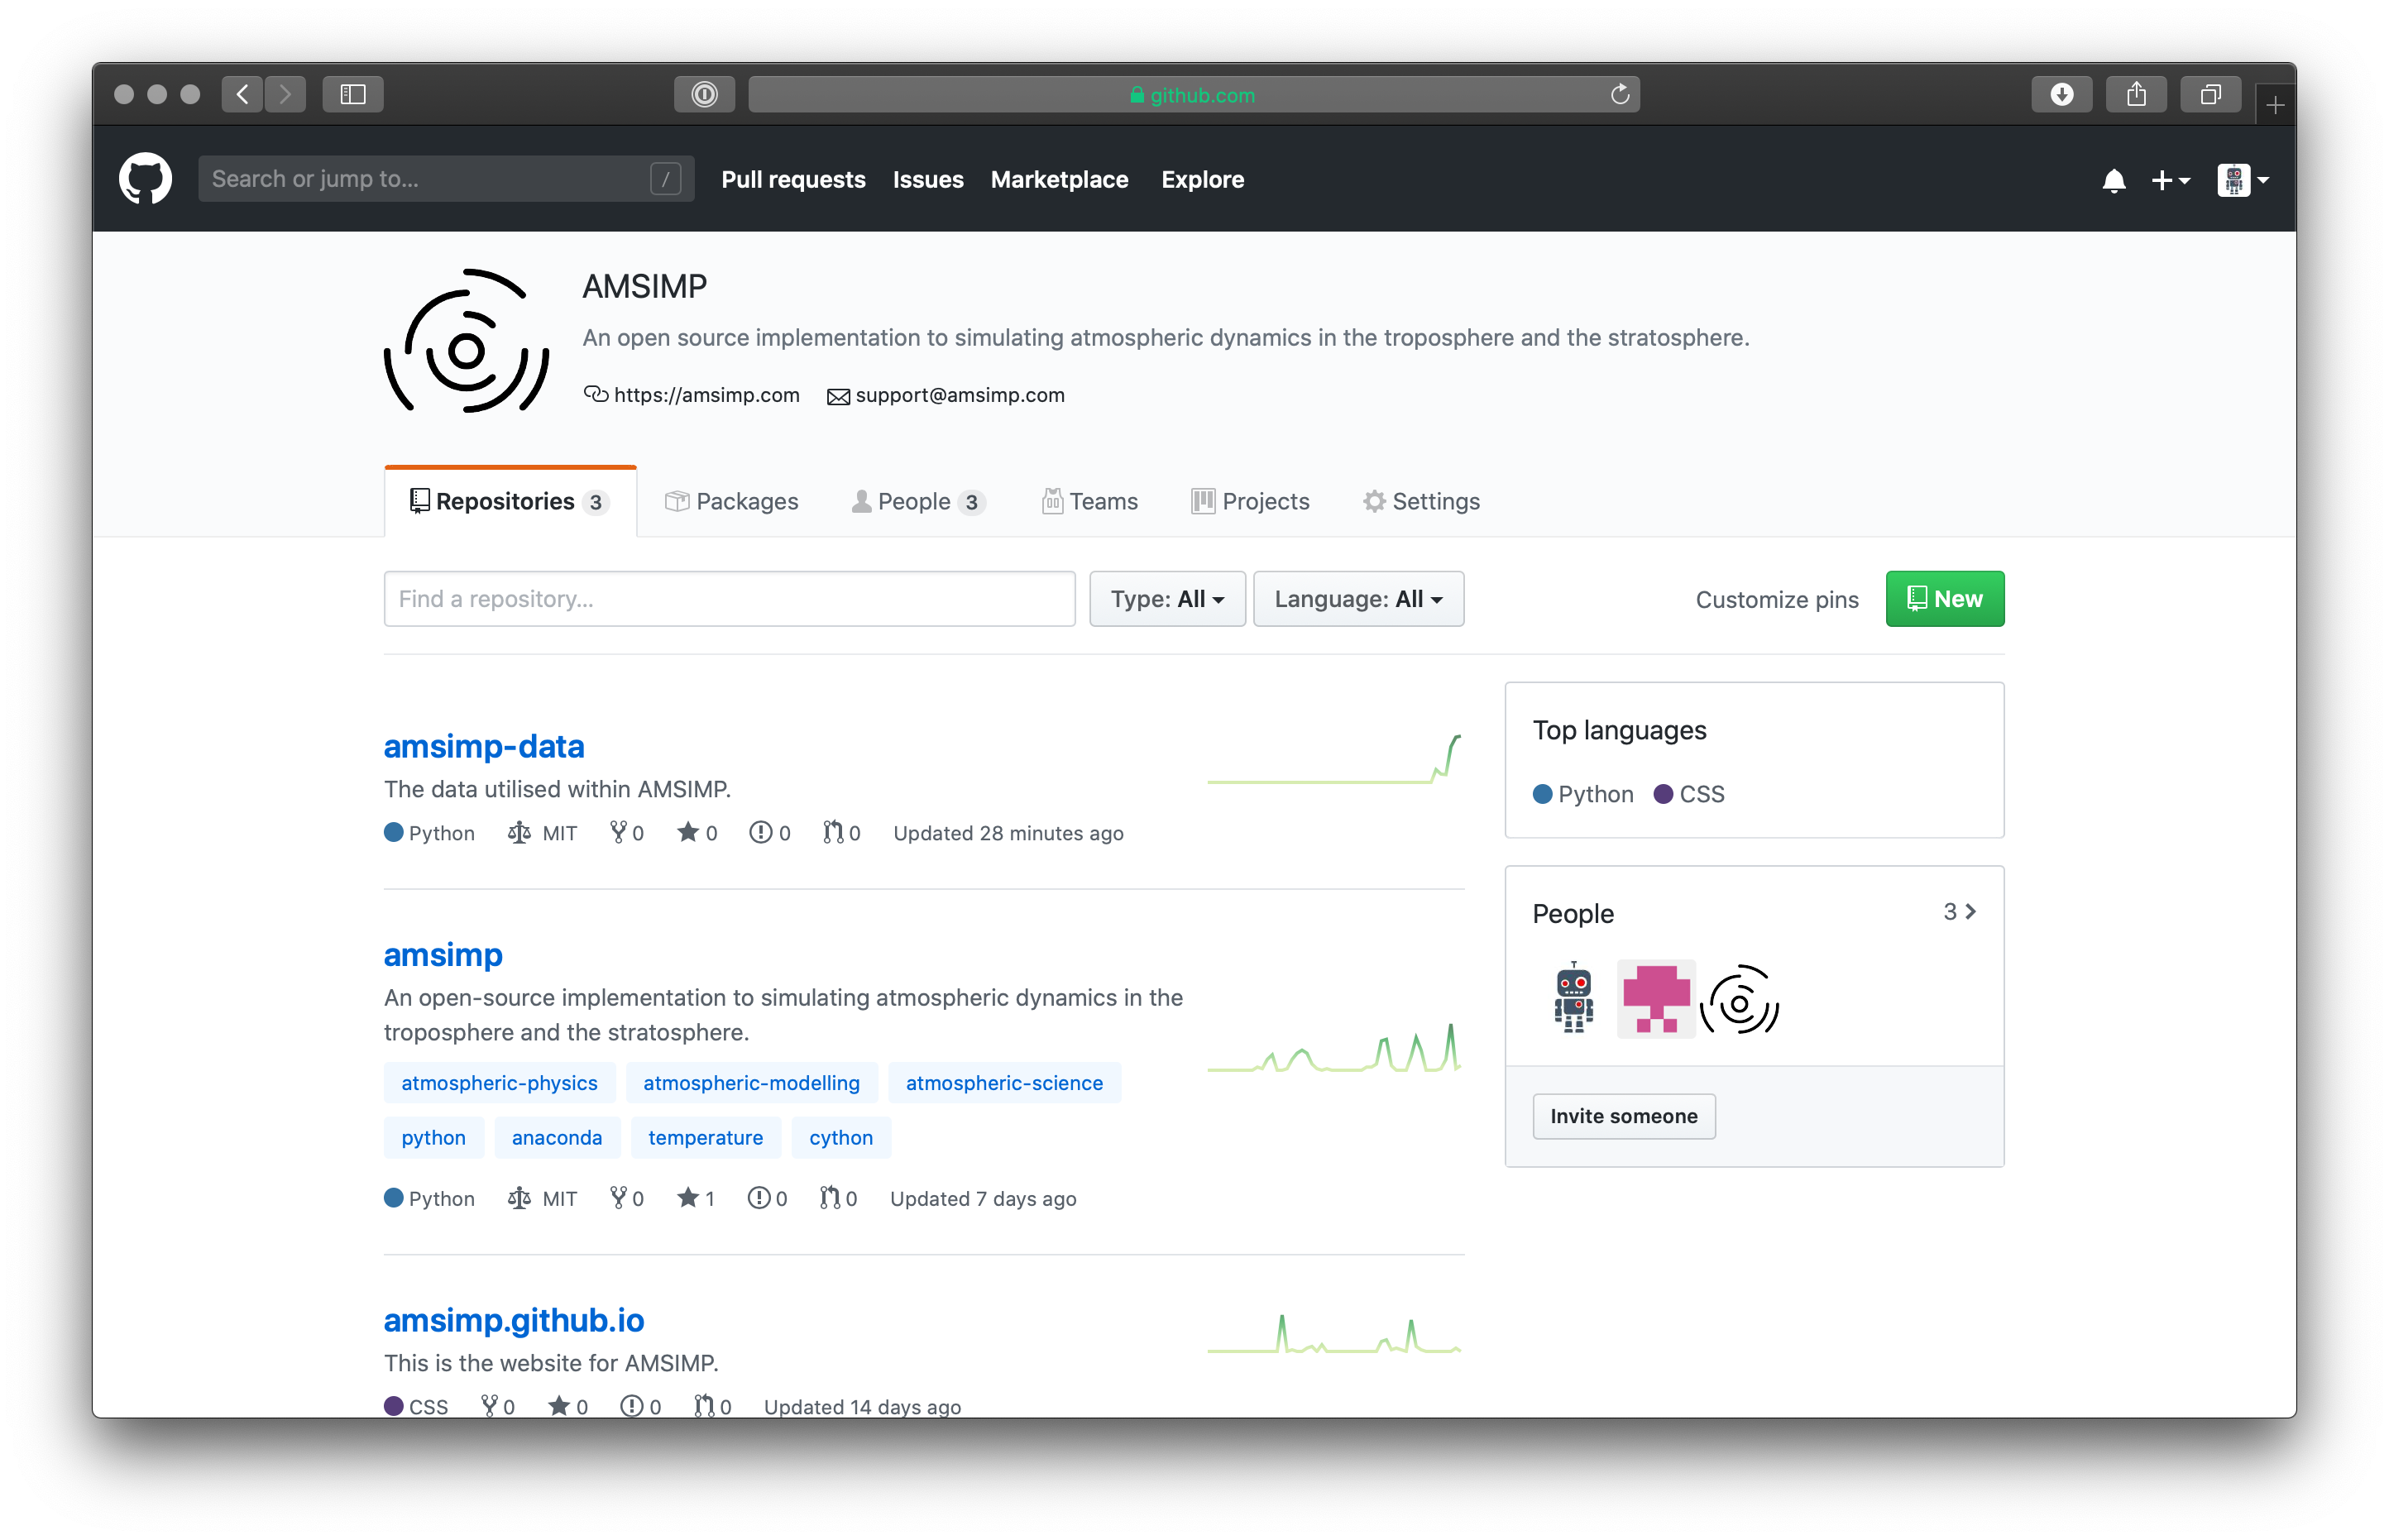
\includegraphics[width=.8\linewidth]{Images/github}
    \caption{A screenshot of the AMSIMP organisation, hosted by the open source platform known as GitHub.}
    \label{github}
\end{figure}

\section{Language Selection}
\subsection{Initial Language Selection}
The most crucial element of this project was choosing an appropriate programming language for the task. During the initial consideration period, I analysed two different programming languages: JavaScript, and Python\cite{python}. 

Initially, I considered the programming language, JavaScript with a run-time environment known as Node.js (Node.js executes code outside of a browser), for two reasons primarily:

\begin{itemize}
    \item JavaScript excels at data visualisation.
    \item Node.js is extremely well suited for memory intensive activities.
\end{itemize}

In line with the expectation of using this programming language, Miss Abbott, and I attended the Dublin Node.js Meetup on the 28th of February. I did this in order to gain an understanding of what Node.js is used for, and what would be the best way one would go about using it. 

In the end, however, I ultimately chose Python for the task due to a number of shortcomings on the part of JavaScript (Node.js), and advantages on the part of Python. Firstly, JavaScript just doesn’t have the same enormous suite of scientific packages and inbuilt functionality that Python does. Using JavaScript, therefore, would waste valuable development time, and ultimately would be entirely inefficient.

Secondly, Python already has an extensive ecosystem with how-to’s available for almost any scientific task you would ever want to do. For JavaScript, this is simply not the case.\cite{javascript_vs_python}

\subsection{Switching to Cython}
During the continued development of the software over the summer months, I discovered a rather severe bottleneck as a result of my choice of programming language: the execution time performance. The culprit behind this bottleneck was a result of Python's dynamically typed nature. Generally, you can classify programming languages into two categories: dynamically typed languages and statically typed languages. 

\begin{definition}
A dynamically typed language is one in which the type of the variable is not known at compile time, and generally, you can define a variable as an integer type at the start of the program for example and later redefine it as a string type. 
\end{definition}

On the other hand, a statically typed language is a language where the type of variable is known at compile time, and during the execution of the program, the variable type must remain constant. 

\hfill

\begin{figure}[H]
    \centering
    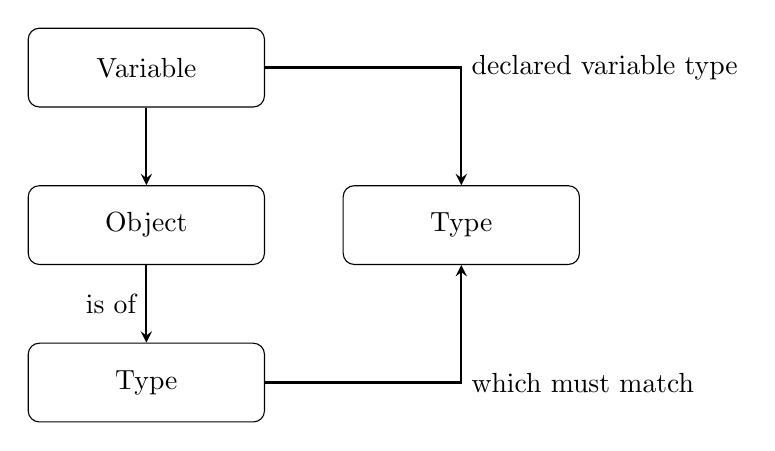
\begin{tikzpicture}[node distance=2cm]
        \tikzstyle{startstop} = [rectangle, rounded corners, minimum width=3cm, minimum height=1cm,text centered, draw=black]
        \tikzstyle{arrow} = [thick,->,>=stealth]
        
        \node (start) [startstop] {Variable};
        \node (obj) [startstop, below of=start] {Object};
        \node (type1) [startstop, right of=obj, xshift=2cm] {Type};
        \node (type2) [startstop, below of=obj] {Type};
        
        \draw [arrow] (start) -- (obj);
        \draw [arrow] (start) -| node[anchor=west] {declared variable type} (type1);
        \draw [arrow] (obj) -- node[anchor=east] {is of} (type2);
        \draw [arrow] (type2) -| node[anchor=west] {which must match} (type1);
    \end{tikzpicture}
    \caption{How statically typed languages handle variables.}
\end{figure}

A statically typed language is particularly useful for software with a large number of loops, or repetitive calculations contained within them. During a loop, a dynamically typed language will continuously check the type of variable after each loop, even if it has done so in previous loops. In a small number of loops, this has a negligible impact on the execution time; however, in a large enough quantity, this has a cumulative effect, significantly stifling the execution time performance. Generally, a piece of software written in a statically typed language will execute a lot faster; this fact will be demonstrated in chapter \ref{6}. The reason behind picking Cython over other statically typed languages, such as C, is that Cython retains all the benefits of Python, with its extensive scientific package library and its simple syntax, while gaining the performance benefits of a statically typed language.



\chapter{Benchmarking}\label{5}
\epigraph{``It's known in theory that log(log(n)) approaches infinity, but no one has ever observed it in practice."}{Grant Sanderson}

To prove the hypothesis that `it is possible to create open source software implementation to simulating atmospheric dynamics, with a recurrent neural network and ensemble prediction system being used in combination with a physical model, that such a software implementation has a reasonable execution time to forecast length ratio, and to determine if such an implementation has a statistically significant accuracy improvement over a traditional deterministic physical model', it is necessary to carry out a series of appropriate benchmarks.

It was determined that it was necessary to carry out a series of appropriate benchmarking within the areas of performance, and accuracy. The performance benchmark would demonstrate whether or not the software has a reasonable execution time to forecast length ratio, and the accuracy benchmark would highlight whether or not the forecasts produced by the software had a reasonable level of accuracy. Considering there is no open source software to which one can compare the software, it was determined that the software would be compared against a proprietary implementation. For this purpose, OpenWeatherAPI was selected as the most appropriate option as it provides accurate data for slightly longer time ranges than other similar application programming interfaces\cite{owa}. 

Please note that all of the benchmarking code is available on the AMSIMP repository, which can be accessed using the following url: \url{https://github.com/amsimp/initial-conditions}

\section{Performance Benchmark}
One of the most important factors to consider when benchmarking a piece of software is the execution time of said software. A piece of software can be as precise and accurate as it wants, however, it isn't of much practical use if it takes the length of time until the heat death of the universe to finish executing. For example, attempting to brute force a 12 character alphanumeric password might work, however, it would take approximately two centuries based on the current capabilities of computers. Considering simulating atmospheric dynamics requires a significant amount of computational resources, it was deemed necessary to run the software on a virtual machine. Using a virtual machine also allows for easier replication and duplication of results, especially considering the wide variety of computer hardware available today. Google's Compute Engine was ultimately chosen as it provided the most flexibility, with the amount of promotional credit being significantly greater than the competition. Without the promotional credit, the benchmarking process would have been an extremely expensive affair to complete (the hardware specification below would have cost approximately one dollar an hour). It was also deemed the only feasible option available due to the restrictions imposed by the COVID-19 pandemic. 

\subsection{Hardware Specifications}\label{specs}
\begin{center}
\begin{tabular}{|c|c|} 
 \hline
  & Compute Engine n1-custom-configuration \\
 \hline
 \textbf{vCPUs} & 8 \\
 \hline
 \textbf{Memory} & 128 GB \\
 \hline
 \textbf{Operating System} & Ubuntu 20.04 LTS \\
 \hline
\end{tabular}\par
\bigskip
Table 5.3.: Compute Engine Hardware Specifications
\end{center}

\subsection{Benchmarking Method}
\begin{definition}
Algorithm is a set of mathematical instructions or rules that, especially if given to a computer, will help to calculate an answer to a problem.
\end{definition}

The aspect of the performance that is being benchmarked is the length of time it takes to generate a forecast of a fixed length, and after which, determining in order to determine the ratio between the execution time and the length of the forecast. For this particular experiment, a forecast length of five days was specified. The reason for utilising such a ratio is that it provides a rough estimate of the usability time of a forecast. For example, it would be highly undesirable for the simulation to take several days if the forecast was only a day in length. A small ratio would increase the amount of time a forecast is usable for, and vice versa, for a high ratio. The following algorithm on the next page was created for this purpose.

\begin{algorithm}[H]
    \caption{Performance Algorithm}
    \begin{algorithmic}[1]
        \State $ start \gets $ The time at the start of the experiment (UNIX time).
        \State $ output = scheme(\texttt{scheme-name}) \gets $ Generate a forecast using the selected scheme. 
        \State $ end \gets $ The time at the end of the experiment (UNIX time). 
        \State $ runtime = end - start \gets $ The difference between the start and end variables is the runtime of the selected scheme.
        \State $ forecast\_length \gets $ The fixed length of the generated forecast.
        \State $ratio = \frac{runtime}{forecast\_length}$
    \end{algorithmic}
\end{algorithm}

\section{Accuracy Benchmark}
Accuracy is probably the most important metric when considering the validity of a given forecasting scheme, therefore, extensive benchmarking was carried out in this particular area. The accuracy benchmarks can be broken down into three distinct categories: comparing against a nave forecasting model, comparing the different forecasting schemes found in the software, and comparing the accuracy of the best forecasting scheme in the software with a proprietary forecasting implementation. The fixed length of the forecast was chosen to be five days, as it was deemed to be a good comprise between short and long term forecasting.

\subsection{Mean Absolute Scaled Error}
The first and most important benchmark to consider is the comparison against a naive forecasting model. A naive forecasting model is one that assumes that the given parameter will not change during the duration of the forecast, the given parameter is constant with respect to time. This is done through the utilisation of the mean absolute scaled error. 

\begin{definition}
The mean absolute scaled error is a measure of the accuracy of forecasts. It is the mean absolute error of the forecast values, divided by the mean absolute error of the in-sample one-step naive forecast.
\end{definition}

The mean absolute scaled error has the following desirable properties:

\begin{itemize}
    \item The mean absolute scaled error penalises positive and negative forecast errors equally, and penalises errors in large forecasts and small forecasts equally. In contrast, the mean absolute percentage error and median absolute percentage error fail both of these criteria, while the "symmetric" sMAPE and sMdAPE fail the second criteria.
    \item The mean absolute scaled error can be easily interpreted, as values greater than one indicate that in-sample one-step forecasts from the naive method perform better than the forecast values under consideration.
\end{itemize}

The following algorithm was developed with the intention to calculate the mean absolute scaled error of a given forecasting scheme, and for the comparison of said forecasting scheme with the naive forecasting model:

\begin{algorithm}[H]
    \caption{Comparison against the Naive Forecasting Model Algorithm}
    \begin{algorithmic}[1]
        \State $ forecast \gets $ The forecasted atmospheric conditions for the next five days. 
        \State $ actual \gets $ The actual atmospheric conditions for the forecast period.
        \State $ naive \gets $ The naive forecasting prediction (it is constant).
        \Function{benchmark}{$forecast, actual, naive$}
            \State $MAE_{forecast} = abs(actual - forecast)$
            \State $MAE_{naive} = abs(actual - naive)$
            \State $MASE = \frac{MAE_{forecast}}{MAE_{naive}}$
        \EndFunction
    \end{algorithmic}
\end{algorithm}

\subsection{Comparison of Schemes}
The second benchmark involves the comparison of the various forecasting schemes available within the software. The available schemes that will be benchmarked are listed as follows: the physical model, the physical with the recurrent neural network enabled, the physical model with the ensemble forecasting system enabled. In the case of the ensemble forecasting system, the mean of the ensemble forecasting system will be utilised rather than any particular ensemble member. The ensemble mean normally verifies better than the control forecast by most standard verification scores because it smooths out unpredictable detail and simply presents the more predictable elements of the forecast\cite{intro_efs}. The comparison metric will be the mean squared error.

For this benchmark, what will be determined is whether the null hypothesis can be rejected or accepted. The null hypothesis $H_0$ is that there is not a significantly significant difference between two given forecasting schemes, while the alternate hypothesis $H_A$ is that there is a significantly significant difference between two given forecasting schemes. This will be determined using a two-sample independent t-test. This can be represented mathematically as the following:

\begin{equation}
    H_0 : \mu_1 = \mu_2 
\end{equation}

\begin{equation}
    H_A : \mu_1 \neq \mu_2 
\end{equation}

\begin{definition}
The independent t-test is an inferential statistical test that determines whether there is a statistically significant difference between the means in two groups.
\end{definition}

To do this, a significance level needs to be set that allows us to either reject or accept the alternative hypothesis. For the purposes of this project, this significance level will be 0.1. The algorithm for this benchmark is pretty similar to algorithm 2, and is as follows:

\begin{algorithm}[H]
    \caption{Comparison of Schemes Algorithm}
    \begin{algorithmic}[1]
        \State $ forecast_{1} \gets $ The forecasted atmospheric conditions for the next five days for a given scheme. 
        \State $ actual_{1} \gets $ The actual atmospheric conditions for the forecast period for a given scheme.
        \State $ forecast_{2} \gets $ The forecasted atmospheric conditions for the next five days for the comparison scheme. 
        \State $ actual_{2} \gets $ The actual atmospheric conditions for the forecast period for the comparison scheme.
        \State $MSE_{1} = (actual_{1} - forecast_{1})^2 \gets$ The mean squared error for the first scheme.
        \State $MSE_{2} = (actual_{2} - forecast_{2})^2 \gets$ The mean squared error for the second scheme.
        \State $p = ttest\_ind(MSE_{1}, MSE_{2}) \gets $ Determines the significance level.
    \end{algorithmic}
\end{algorithm}

\subsection{Comparison against OpenWeatherAPI}
The final benchmark will involve the comparison of the software's most accurate scheme against a proprietary implementation. The proprietary implementation ultimately chosen was OpenWeatherAPI, due to the fact that, as previously mentioned, it provides accurate data for slightly longer time ranges than other similar application programming interfaces\cite{owa}. The algorithm is the exact same as algorithm, just slightly edited to incorporate data from OpenWeatherAPI.  

\begin{algorithm}[H]
    \caption{Comparison against OpenWeatherAPI Algorithm}
    \begin{algorithmic}[1]
        \State $ forecast_{1} \gets $ The forecasted atmospheric conditions for the next five days for the software's most accurate scheme. 
        \State $ actual_{1} \gets $ The actual atmospheric conditions for the forecast period for for the software's most accurate scheme.
        \State $ forecast_{2} \gets $ The forecasted atmospheric conditions for the next five days for OpenWeatherAPI. 
        \State $ actual_{2} \gets $ The actual atmospheric conditions for the forecast period for the OpenWeatherAPI.
        \State $MSE_{1} = (actual_{1} - forecast_{1})^2 \gets$ The mean squared error for the software's forecast.
        \State $MSE_{2} = (actual_{2} - forecast_{2})^2 \gets$ The mean squared error for OpenWeatherAPI's forecast.
        \State $p = ttest\_ind(MSE_{1}, MSE_{2}) \gets $ Determines the significance level.
    \end{algorithmic}
\end{algorithm}


\chapter{Results}\label{6}
\epigraph{``Of course it is happening inside your head, Harry, but why on earth should that mean it is not real?"}{Albus Dumbledore}

\section{Performance Benchmark}
\begin{figure}[H]
    \centering
    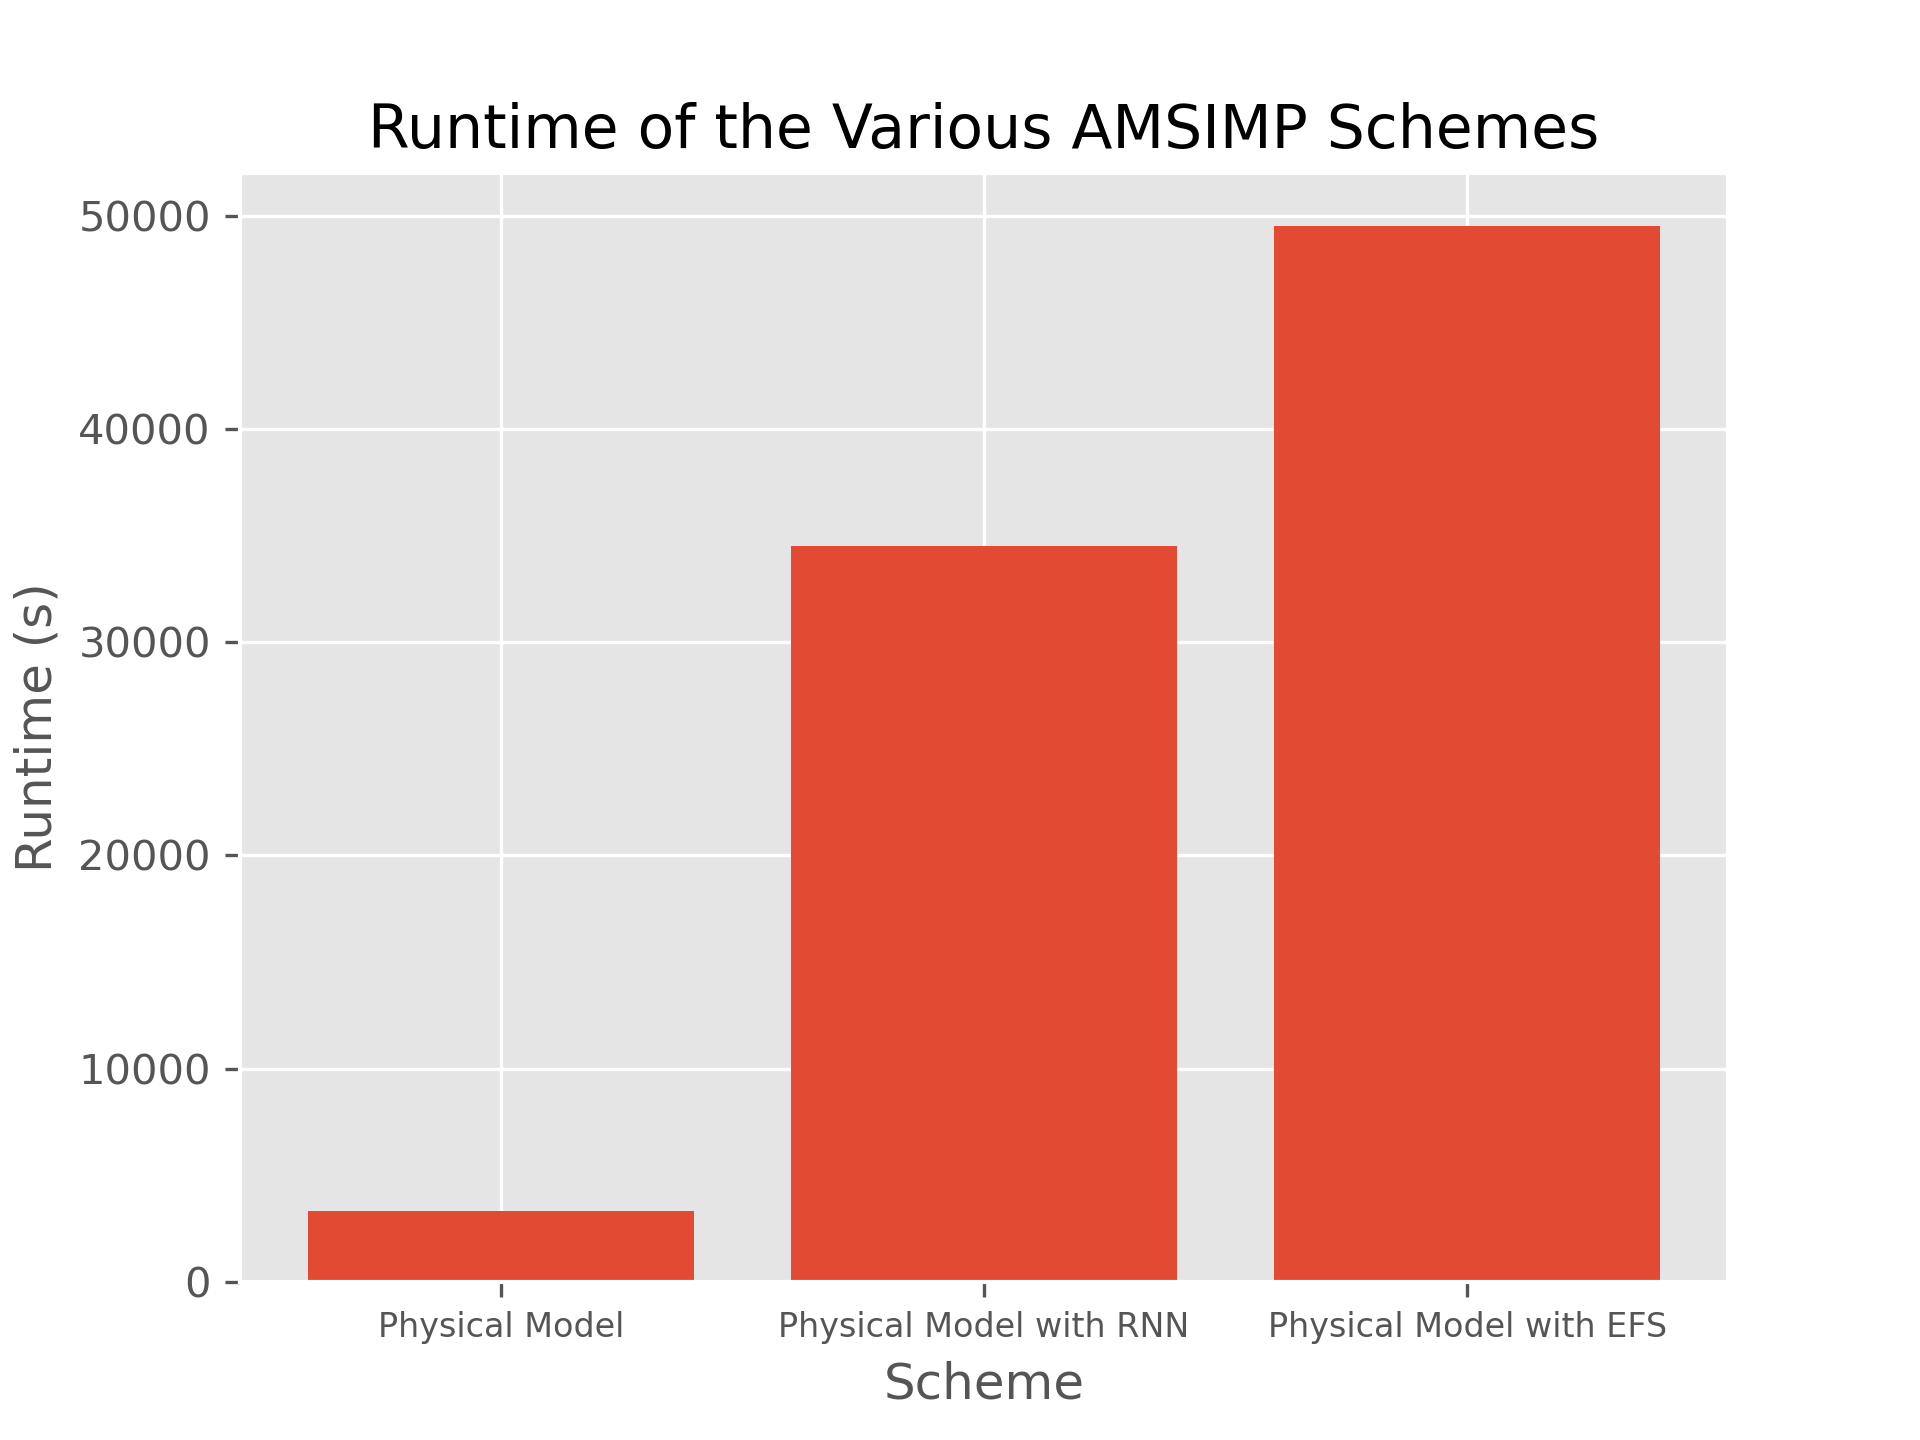
\includegraphics[width=.8\linewidth]{Graphs/performance/runtime.png}
    \caption{Runtime of Various AMSIMP Schemes}
\end{figure}

\begin{figure}[H]
    \centering
    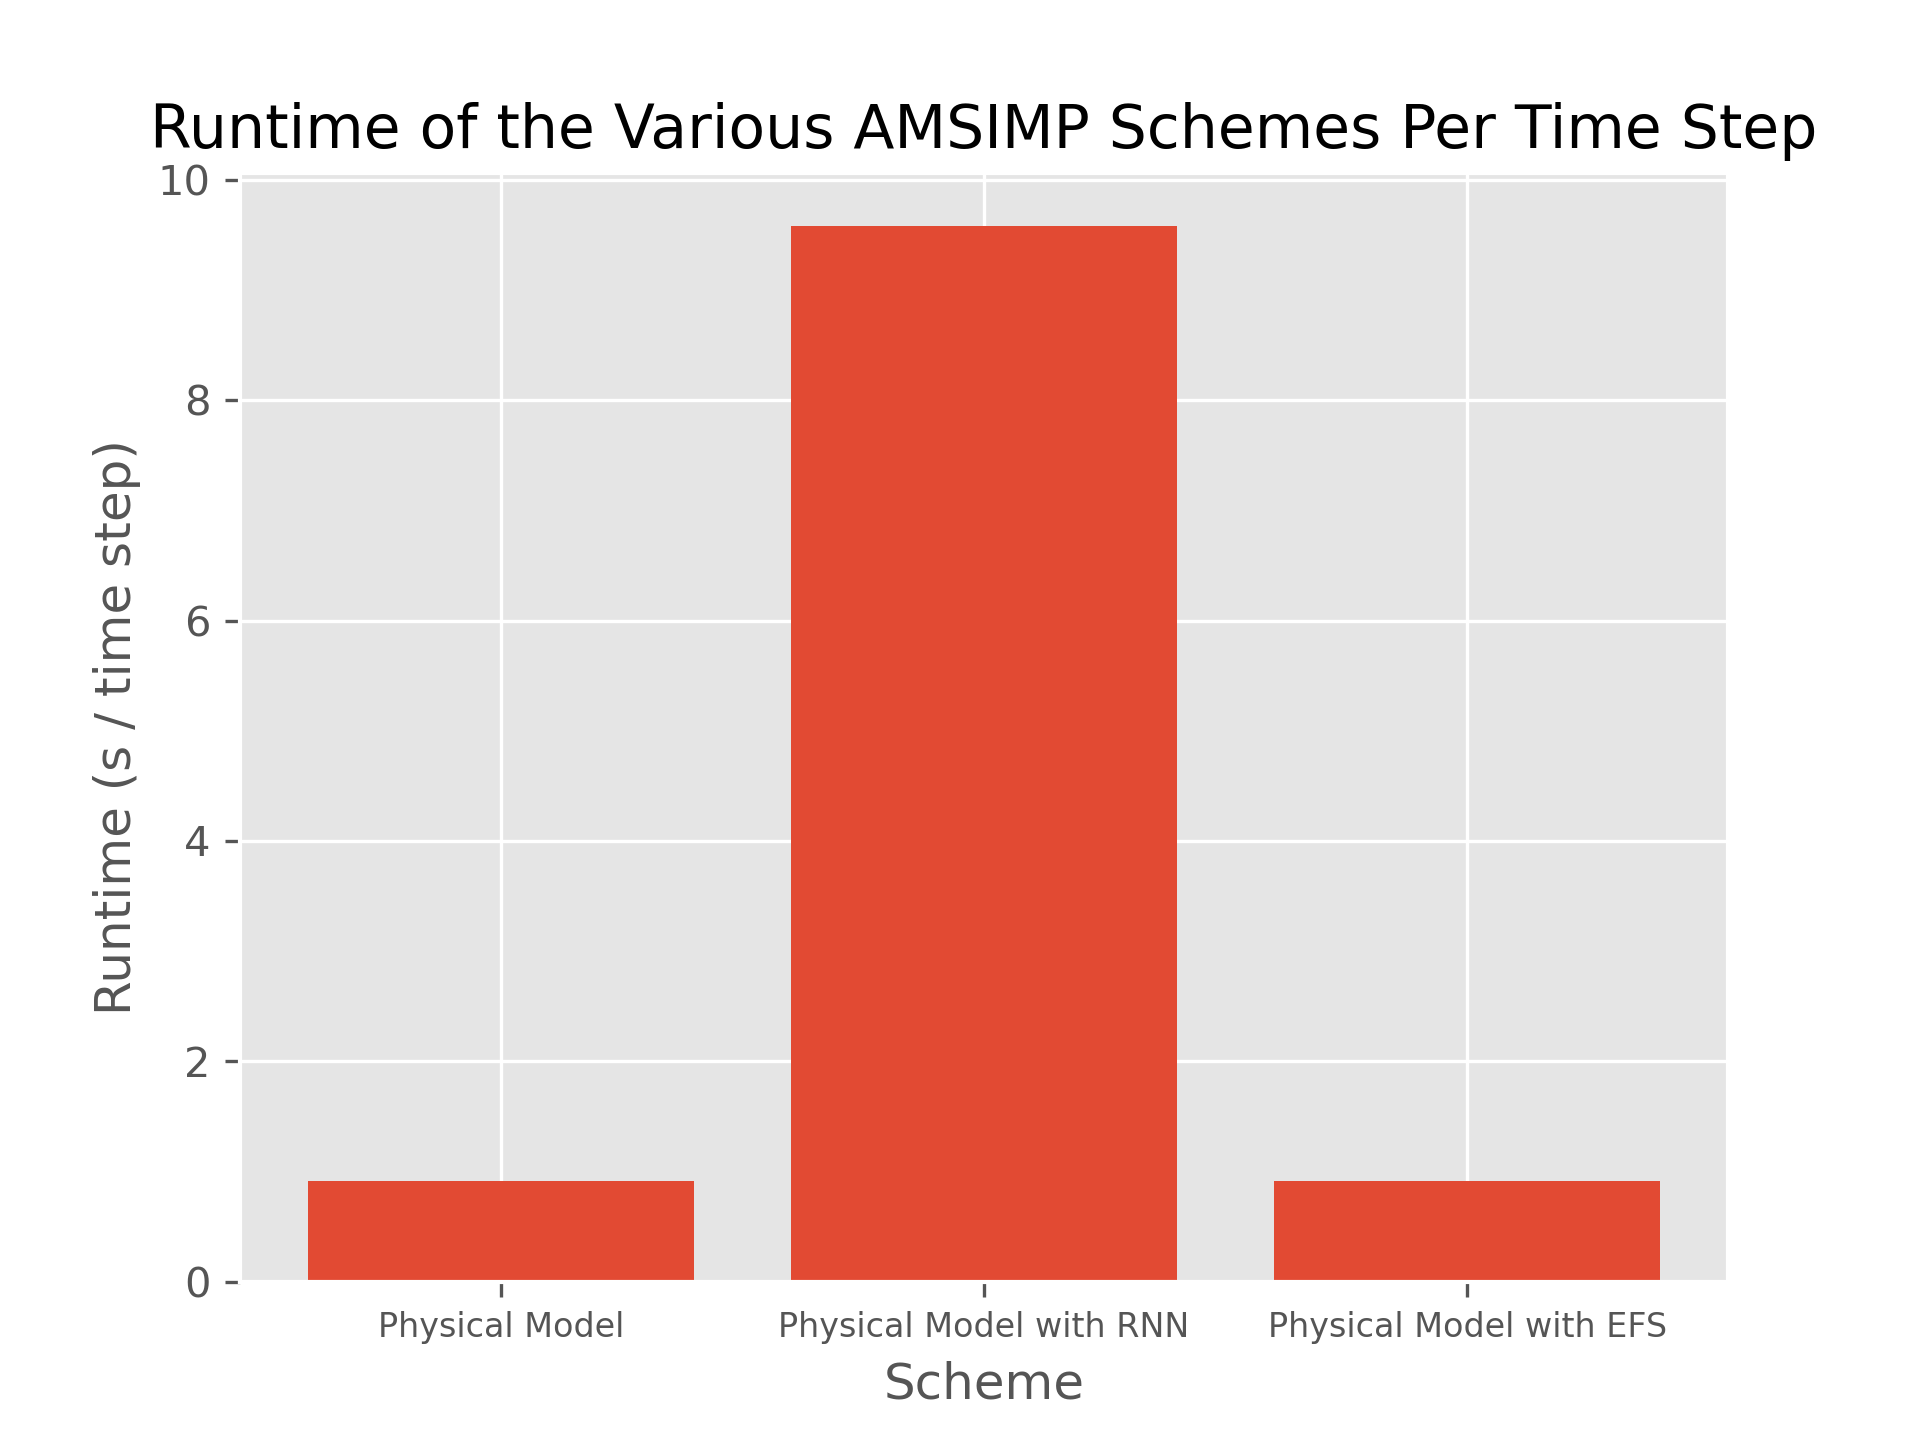
\includegraphics[width=.8\linewidth]{Graphs/performance/runtime_per_timestep.png}
    \caption{Runtime of Various AMSIMP Schemes Per Time Step}
\end{figure}

\begin{figure}[H]
    \centering
    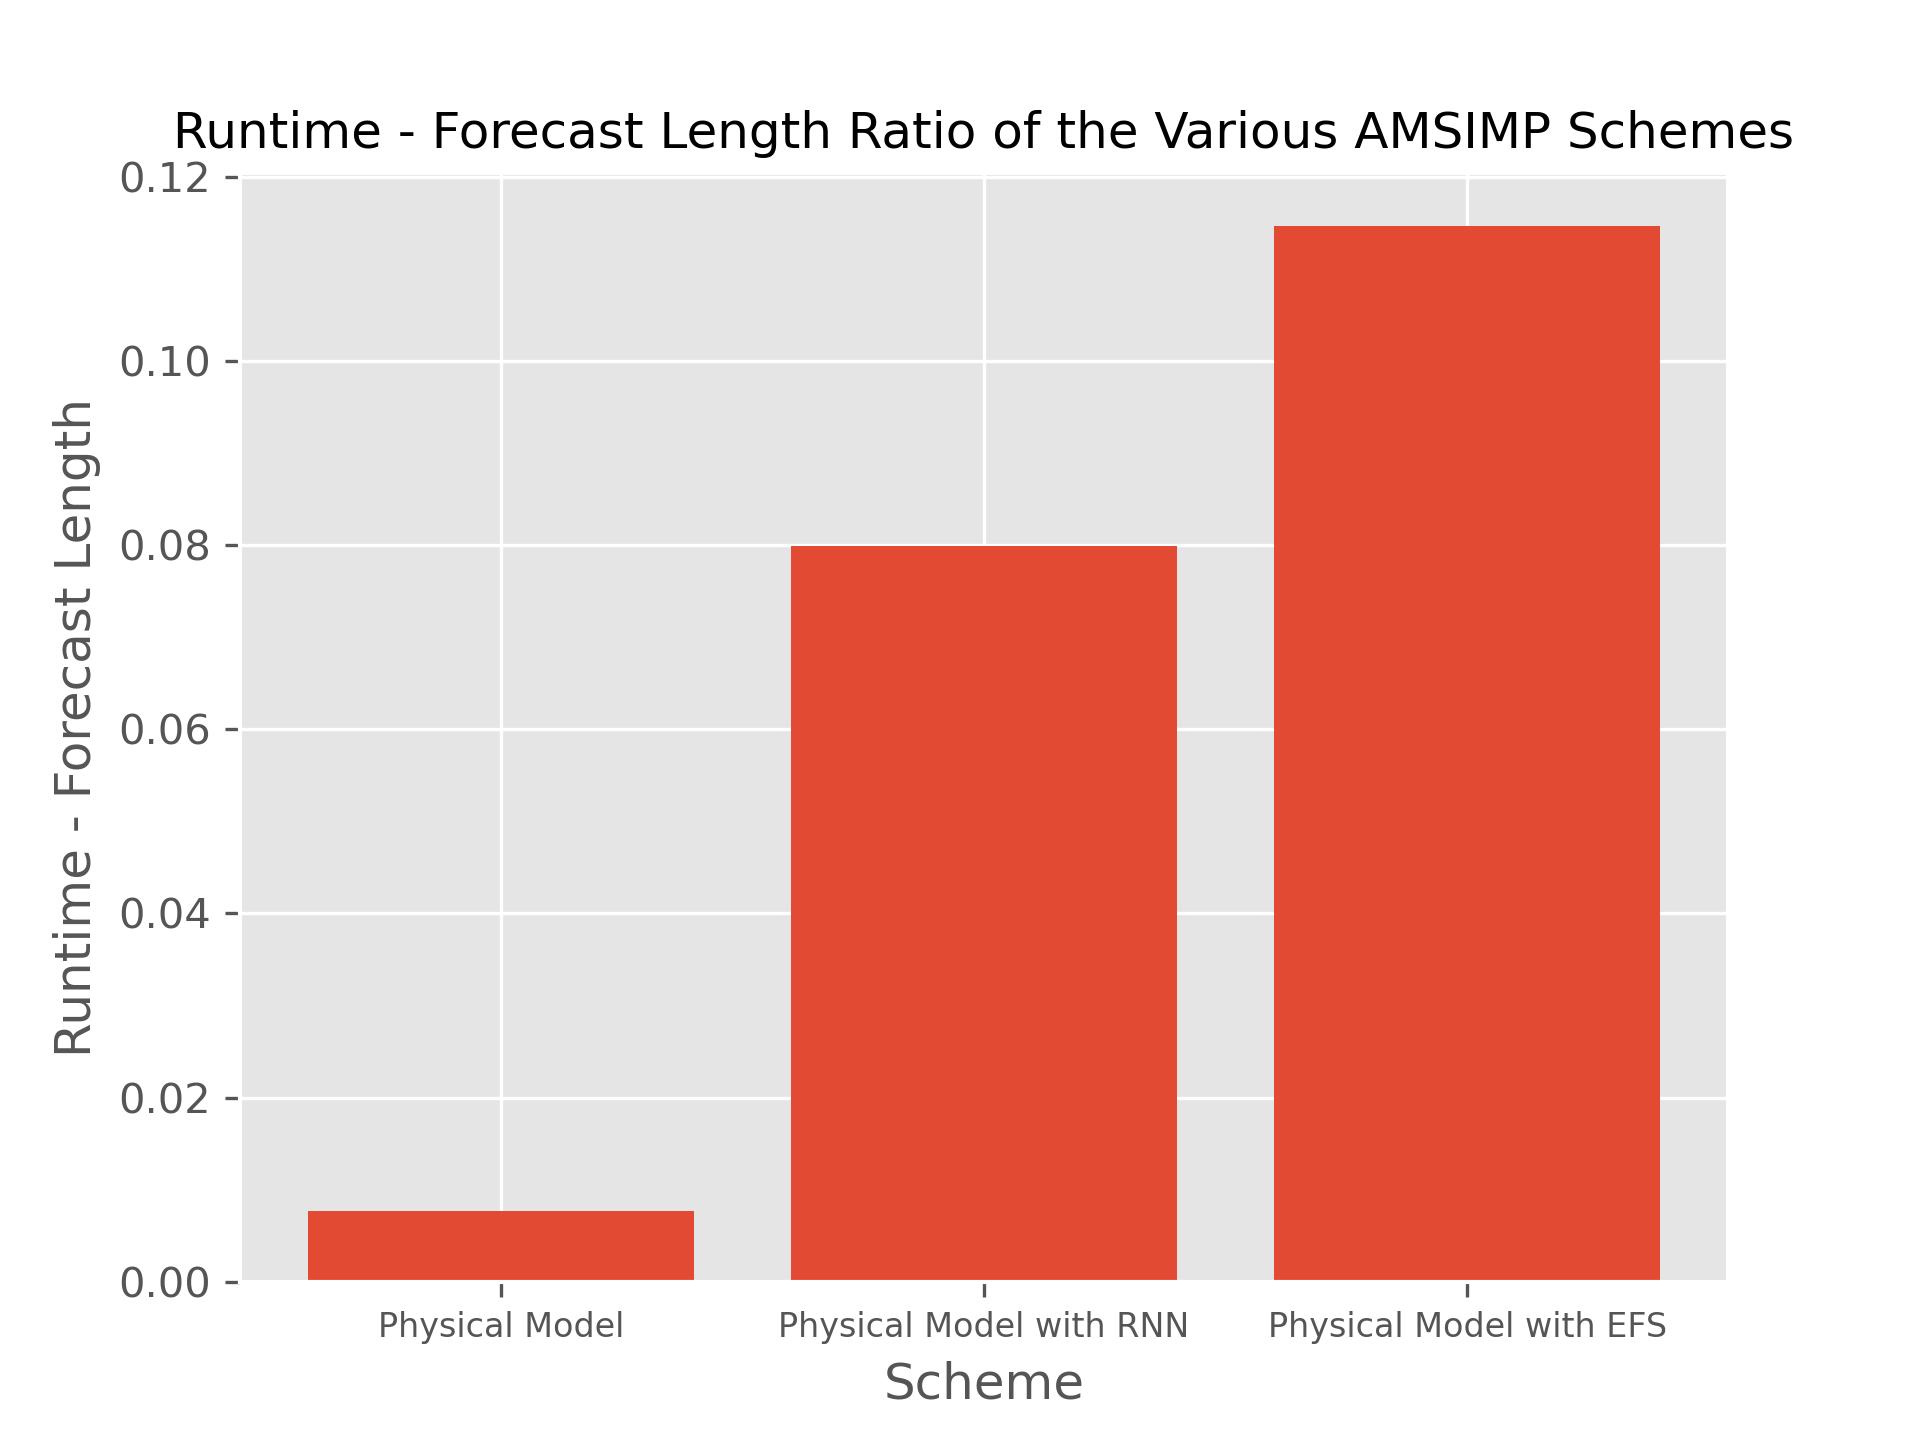
\includegraphics[width=.8\linewidth]{Graphs/performance/ratio.png}
    \caption{Runtime - Forecast Length Ratio of the Various AMSIMP Schemes}
\end{figure}

\section{Accuracy Benchmark}
\subsection{Mean Absolute Scaled Error}
\begin{figure}[H]
    \centering
    \includegraphics[width=.7\linewidth]{Graphs/accuracy/mase/temperature.png}
    \caption{AMSIMP Air Temperature Mean Absolute Scaled Error}
\end{figure}

\begin{figure}[H]
    \centering
    \includegraphics[width=.7\linewidth]{Graphs/accuracy/mase/virtual_temperature.png}
    \caption{AMSIMP Virtual Temperature Mean Absolute Scaled Error}
\end{figure}

\begin{figure}[H]
    \centering
    \includegraphics[width=.8\linewidth]{Graphs/accuracy/mase/relative_humidity.png}
    \caption{AMSIMP Relative Humidity Mean Absolute Scaled Error}
\end{figure}

\begin{figure}[H]
    \centering
    \includegraphics[width=.8\linewidth]{Graphs/accuracy/mase/geopotential_height.png}
    \caption{AMSIMP Geopotential Height Mean Absolute Scaled Error}
\end{figure}

\begin{figure}[H]
    \centering
    \includegraphics[width=.8\linewidth]{Graphs/accuracy/mase/zonal_wind.png}
    \caption{AMSIMP Zonal Wind Mean Absolute Scaled Error}
\end{figure}

\begin{figure}[H]
    \centering
    \includegraphics[width=.8\linewidth]{Graphs/accuracy/mase/meridional_wind.png}
    \caption{AMSIMP Meridional Wind Mean Absolute Scaled Error}
\end{figure}

\subsection{Comparison of Schemes}
\begin{figure}[H]
    \centering
    \includegraphics[width=.8\linewidth]{Graphs/accuracy/comparsion_schemes/temperature.png}
    \caption{AMSIMP Air Temperature Mean Squared Error}
\end{figure}

\begin{figure}[H]
    \centering
    \includegraphics[width=.8\linewidth]{Graphs/accuracy/comparsion_schemes/virtual_temperature.png}
    \caption{AMSIMP Virtual Temperature Mean Squared Error}
\end{figure}

\begin{figure}[H]
    \centering
    \includegraphics[width=.8\linewidth]{Graphs/accuracy/comparsion_schemes/relative_humidity.png}
    \caption{AMSIMP Relative Humidity Mean Squared Error}
\end{figure}

\begin{figure}[H]
    \centering
    \includegraphics[width=.8\linewidth]{Graphs/accuracy/comparsion_schemes/geopotential_height.png}
    \caption{AMSIMP Geopotential Height Mean Squared Error}
\end{figure}

\begin{figure}[H]
    \centering
    \includegraphics[width=.8\linewidth]{Graphs/accuracy/comparsion_schemes/zonal_wind.png}
    \caption{AMSIMP Zonal Wind Mean Squared Error}
\end{figure}

\begin{figure}[H]
    \centering
    \includegraphics[width=.8\linewidth]{Graphs/accuracy/comparsion_schemes/meridional_wind.png}
    \caption{AMSIMP Meridional Wind Mean Squared Error}
\end{figure}

\subsection{Comparison against OpenWeatherAPI}
\begin{figure}[H]
    \centering
    \includegraphics[width=.8\linewidth]{Graphs/accuracy/comparsion_openweatherapi/temperature.png}
    \caption{Air Temperature Mean Squared Error}
\end{figure}

\begin{figure}[H]
    \centering
    \includegraphics[width=.8\linewidth]{Graphs/accuracy/comparsion_openweatherapi/virtual_temperature.png}
    \caption{Virtual Temperature Mean Squared Error}
\end{figure}

\begin{figure}[H]
    \centering
    \includegraphics[width=.8\linewidth]{Graphs/accuracy/comparsion_openweatherapi/relative_humidity.png}
    \caption{Relative Humidity Mean Squared Error}
\end{figure}

\begin{figure}[H]
    \centering
    \includegraphics[width=.8\linewidth]{Graphs/accuracy/comparsion_openweatherapi/zonal_wind.png}
    \caption{Zonal Wind Mean Squared Error}
\end{figure}

\begin{figure}[H]
    \centering
    \includegraphics[width=.8\linewidth]{Graphs/accuracy/comparsion_openweatherapi/meridional_wind.png}
    \caption{Meridional Wind Mean Squared Error}
\end{figure}

\chapter{Conclusions}\label{7}
\epigraph{``It is our choices, Harry, that show what we truly are, far more than our abilities."}{Albus Dumbledore}

The previous chapters have discussed the development of an open source implementation to improve numerical weather prediction through the utilisation of a neural network architecture. Although extremely time consuming, the importance of an open source implementation cannot be understated. It could potentially open up a field to a wider group, and often doesn't receive the media attention it rightfully deserves. 

Future applications of this work are extremely wide ranging, from usage in numerical weather prediction schemes that take in observational data collected from satellites, and ground stations in order to provide a picture of future weather events; to forming a starting point in future research of atmospheric phenomena. While, at the moment, it definitely would be inaccurate to say the software is ready for such usage, with future enhancements which I will touch on in a minute, it most certainly will.

\section{Looking Back}
To prove the hypothesis that `it is possible to train a neural network on an atmospheric reanalysis dataset based on data from the 10 years, that such a neural network captures crucial weather patterns, and can predict the future evolution of the atmosphere, and that such a machine learning model will ultimately improve numerical weather prediction in comparison to established physics-based models.', it was necessary to carry out a series of appropriate benchmarks.

\subsection{Analysis of Results}
This report hypothesises that it is possible to train a neural network on an atmospheric reanalysis dataset based on data from the 10 years, that such a neural network captures crucial weather patterns, and can predict the future evolution of the atmosphere, and that such a machine learning model will ultimately improve numerical weather prediction in comparison to established physics-based models.

To gain an insight into the future feasibility of neural networks in the field of meteorology, a comparison between the performance of the current model against the performance of the previous LSTM model is shown in section \ref{old_model}. Air temperature is the only parameter examined for this comparison, as the previous model did not incorporate geopotential. Concerning the two metrics, root mean squared error and mean absolute error, there has been a dramatic performance improvement. There has been a mean decrease of 52.5 \% in the root mean squared error values, and a mean decrease of 48.6 \% in the mean absolute error values; on average a 50.6 \% decrease in error metrics across the board. This demonstrates the continued improvement and enhancement of the models over the last few months; but, it also demonstrates that the performance of the software can still be improved drastically. The performance increase has not reached a plateau, which is extremely promising.

One of the key factors which led to the development of a machine learning model was the expected decrease in computational resources required to generate a forecast. While the initial training of the model was computationally burdensome, particularly with respect to memory, the assumption made at the start of this project holds once the model is trained. Once the model has trained, a performance increase of 6.18 times can be expected in comparison against a physics-based model of a similar resolution, the ECMWF IFS T63. It is also important to note that the benchmark of the software was run on a consumer-grade, MacBook Pro while the benchmark of the ECMWF IFS T63 model was performed on a single XC40 node with 36 cores. Hence, a further increase in performance can be expected with a similar configuration.

With respect to the benchmarking outlined in chapter \ref{benchmarking_chapter}, the forecast system needs to beat the climatology forecast and the persistence forecast to be classified as useful. The benchmarks have demonstrated that the model can be generally regarded as useful, particularly on longer periods and in relation to air temperature, in particular, however, the models generally fail to beat well established physics-based models at this time. The model is significantly better at creating air temperature predictions and appears to suffer with geopotential predictions. The root mean squared error and mean squared error demonstrate that the model's air temperature becomes useful after approximately 24 hours of forecast time, with the model ultimately beating the ECMWF IFS T42 model after approximately 96 hours. The picture for geopotential is less rosy, with the root mean squared error and mean squared error demonstrating that the model's geopotential predictions become useful after approximately 96 hours of forecast time. An interesting point to note is that the error values initially are quite high, the error values appear to plateau. This may suggest that the model may be quite useful at generating climate forecasts. Concerning spatial awareness as measured by the anomaly correlation coefficient, both the mode's geopotential and air temperature predictions become useful after approximately 120 hours of forecast time. The spatial awareness of the model can be generally regarded as quite poor, it appears that the spatial aspect of a weather forecast was not captured by the model. 

Hence, the hypothesis that was proposed has partially been proven and can be accepted, as such.

\subsection{Sources of Error}

Hence, the hypothesis that was proposed has partially been proven, however, there are a few areas which could have hindered the performance of the software or led to a possible source of error:

\begin{itemize}
    \item As mentioned in section \ref{era5_dataset}, it was decided to use a spatial resolution of $1^{\circ}$ ($179 \times 360$ grid points) and a temporal resolution of 2 hours. A lower resolution was chosen in order to reduce the amount of computational resources required to train the model. Through high spatial resolution, however, a forecast can show the effects of local air currents, topography and soil cover. The forecasts produced thereby show local weather differences in more precise way\cite{res}. High resolution produces high precision, hence, while choosing a lower resolution may have lowered the computational burden during training, it may have had a significant on the performance of the model.
\end{itemize}

\section{Looking Ahead}
The software is currently in an alpha release state. An alpha version of any software is a very early version of the software that may not contain all of the features that are planned for the final version\cite{alpha}. In this section, I will briefly outline the enhancements and features that will be released in the beta version of the software, which is planned for release in Spring 2021:

\begin{itemize}
    \item One of the most natural coordinate systems to use on Earth is a latitude‐longitude grid. This was the coordinate system of choice for this project due to its simplicity, but, this system has singularities at the North Pole and South Pole that makes it difficult to use translationally‐invariant convolution operations on this grid. To combat this particular problem in this project, the poles were excluded from the dataset, however, a more elegant solution to preserve spatial locality is to approximate data on the globe using the cubed sphere. This projection has been shown to give more uniformly sized grid cells than the alternative projections and to also produce better solutions to finite‐difference and discontinuous Galerkin approximations to partial differential equations on the sphere. The cubed sphere is used for state‐of‐the‐art NWP such as in the FV3 dynamical core of the National Oceanic and Atmospheric Administration's Global Forecast System model\cite{cubed_sphere}. This is an avenue that will be explored in the coming months. 
    \item As mentioned previously, a high resolution weather forecast produces high precision. As a result, in order to improve the performance of the model, the model will be trained on a higher resolution dataset. At this point, a resolution has not been decided, however, the decision will be made based on the computational resources available to initially train the model and the expected increase in performance that could be made by switching to a higher resolution. 
    \item The three parameters on which the machine learning models were trained upon were: air temperature at 850 hPa, geopotential at 500 hPa, and air temperature at 2 metres above the surface. While these parameters are extremely important to predict from a meteorological point of view, the general public require predictions for the amount of precipitation to be made several days in advance; in order to make personal, and business decisions. This may be supplying shops with more food during periods of snowfall, or county councils setting up flood defences in town. In the coming months, the model will be trained on such parameters in order to provide the most useful weather forecast possible.  
\end{itemize}

\newpage

\pagenumbering{Roman}

\appendix
\renewcommand{\thesection}{\Alph{section}.\arabic{section}}
\setcounter{section}{0}
\begin{appendices}
    \section{Code for the AMSIMP Global Forecast Model}\label{model_code}
    \begin{minted}[mathescape,linenos,frame=lines]{python}
def model(epochs, bs):
    # Number of elements.
    n = len(os.listdir("processed_dataset/"))
    lst_n = np.linspace(1, n, n)
    
    # Define training dataset and validation dataset.
    # Training.
    train_ns = lst_n[:int(0.7 * n)]
    train_generator = DataGenerator(
        train_ns,
        batch_size=bs,
    )
    print("Training dataset created.")
    
    # Validation.
    val_ns = lst_n[int(0.7 * n):int(0.9 * n)]
    val_generator = DataGenerator(
        val_ns, 
        batch_size=bs,
        shuffle=False
    )
    print("Validation dataset created.")
    
    with mirrored_strategy.scope():
        # Create, and train models.
        # Optimiser.
        opt = Adam(lr=1e-3, decay=1e-5)
        # Create model.
        model = Sequential()

        # First layer.
        model.add(
            ConvLSTM2D(
                filters=64, 
                kernel_size=(7, 7),
                input_shape=(6, 179, 360, 3), 
                padding='same', 
                return_sequences=True, 
                activation='tanh', 
                recurrent_activation='hard_sigmoid',
                kernel_initializer='glorot_uniform', 
                unit_forget_bias=True, 
                dropout=0.3, 
                recurrent_dropout=0.3, 
                go_backwards=True
            )
        )
        # Batch normalisation.
        model.add(BatchNormalization())
        # Dropout.
        model.add(Dropout(0.1))
        
        # Second layer.
        model.add(
            ConvLSTM2D(
                filters=32, 
                kernel_size=(7, 7), 
                padding='same', 
                return_sequences=True, 
                activation='tanh', 
                recurrent_activation='hard_sigmoid', 
                kernel_initializer='glorot_uniform', 
                unit_forget_bias=True, 
                dropout=0.4, 
                recurrent_dropout=0.3, 
                go_backwards=True
            )
        )
        # Batch normalisation.
        model.add(BatchNormalization())
        
        # Third layer.
        model.add(
            ConvLSTM2D(
                filters=32, 
                kernel_size=(7, 7), 
                padding='same', 
                return_sequences=True, 
                activation='tanh', 
                recurrent_activation='hard_sigmoid', 
                kernel_initializer='glorot_uniform', 
                unit_forget_bias=True, 
                dropout=0.4, 
                recurrent_dropout=0.3, 
                go_backwards=True
            )
        )
        # Batch normalisation.
        model.add(BatchNormalization())
        # Dropout.
        model.add(Dropout(0.1))

        # Final layer.
        model.add(
            ConvLSTM2D(
                filters=32, 
                kernel_size=(7, 7), 
                padding='same', 
                return_sequences=True, 
                activation='tanh', 
                recurrent_activation='hard_sigmoid', 
                kernel_initializer='glorot_uniform', 
                unit_forget_bias=True, 
                dropout=0.5, 
                recurrent_dropout=0.3, 
                go_backwards=True
            )
        )
        # Batch normalisation.
        model.add(BatchNormalization())

        # Add dense layer.
        model.add(Dense(3))
    
    # Compile model.
    model.compile(
        optimizer=opt, 
        loss='mse'
    )
    # Summary of model.
    model.summary()

    # Train.
    model.fit(
        train_generator,
        validation_data=val_generator,
        epochs=epochs,
        callbacks=[
            tf.keras.callbacks.EarlyStopping(
                monitor="val_loss", min_delta=0, patience=2, mode="auto"
            )
        ],
    )
    
    return model
    \end{minted}
    
    \section{Comparison against Previous Model}\label{old_model}
    \begin{figure}[H]
        \centering
        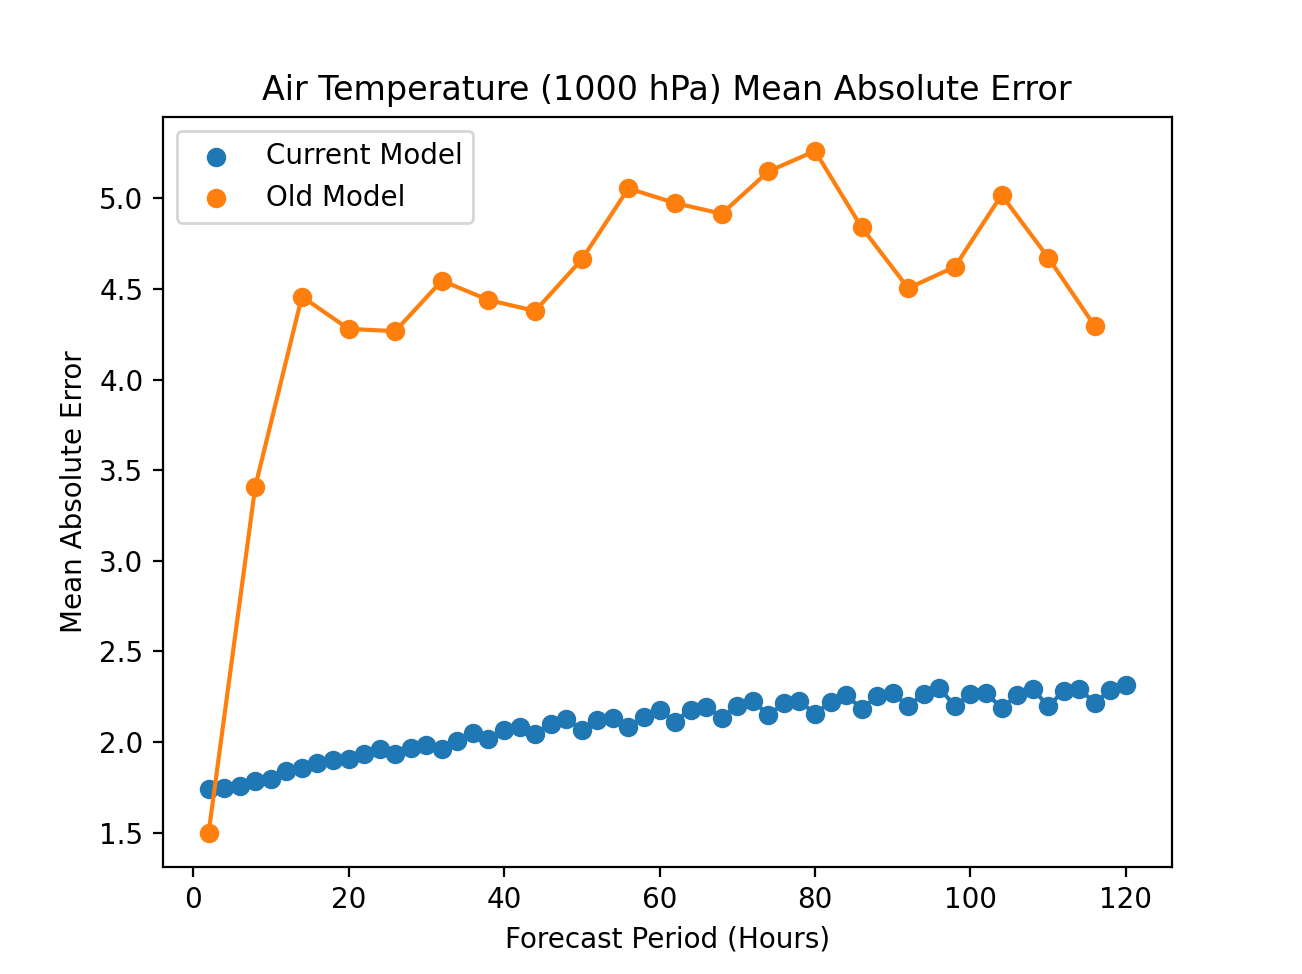
\includegraphics[width=.7\linewidth]{Plots/Results/Temperature/t1000_mae.png}
        \caption{MAE for Air Temperature at 1000 hPa}
    \end{figure}
    
    \begin{figure}[H]
        \centering
        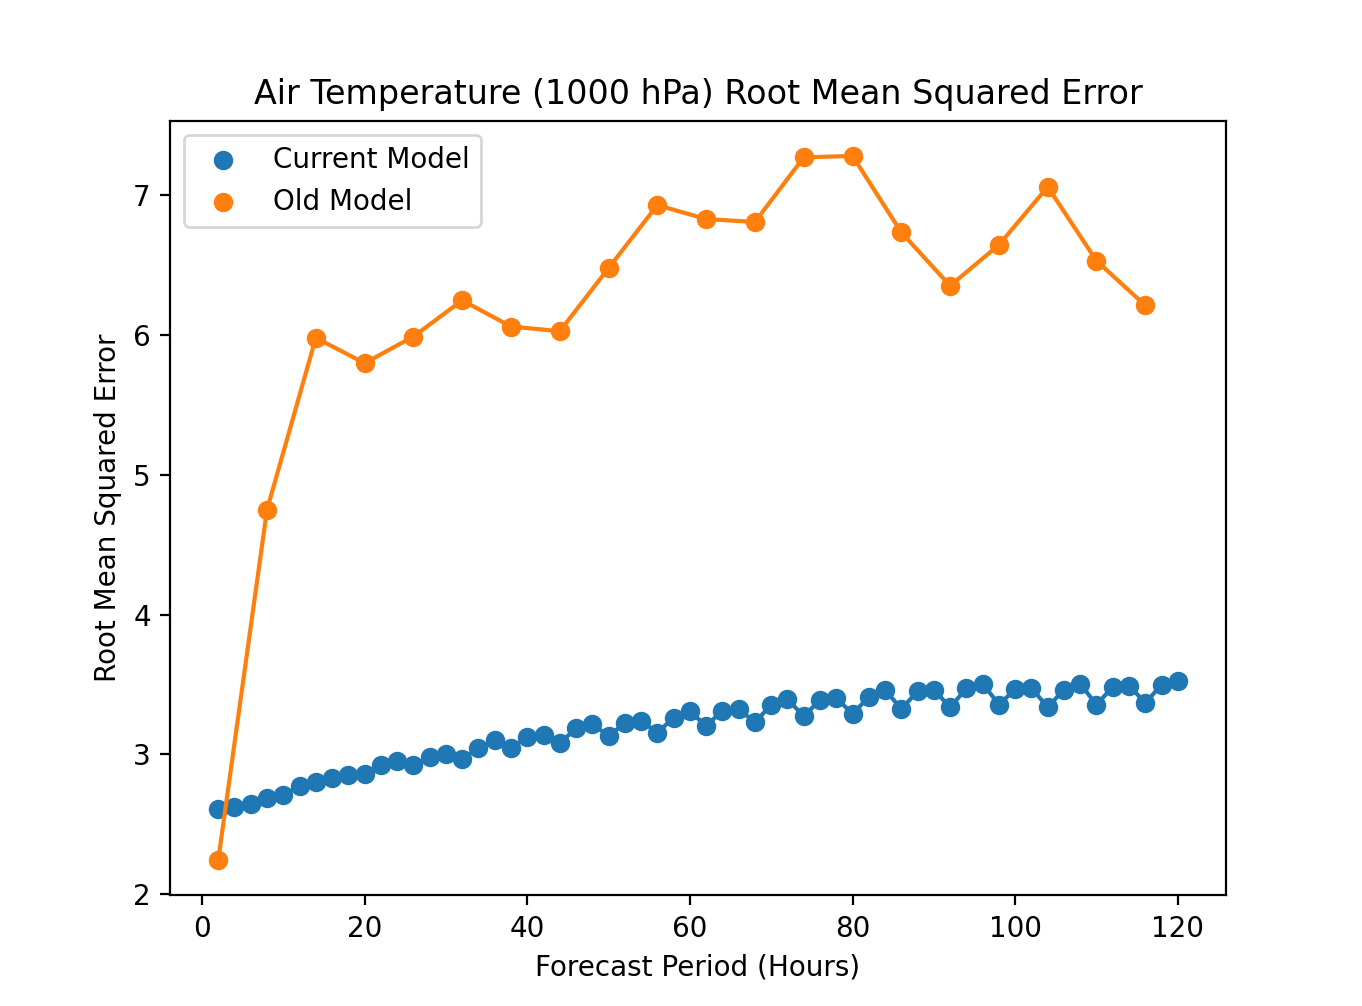
\includegraphics[width=.7\linewidth]{Plots/Results/Temperature/t1000_rmse.png}
        \caption{RMSE for Air Temperature at 1000 hPa}
    \end{figure}
\end{appendices}

\pagenumbering{Roman}

\printbibliography[heading = bibintoc]

\end{document}